%% This is the ctufit-thesis example file. It is used to produce theses
%% for submission to Czech Technical University, Faculty of Information Technology.
%%
%% Get the newest version from
%% https://gitlab.fit.cvut.cz/theses-templates/FITthesis-LaTeX
%%
%%
%% Copyright 2021, Eliska Sestakova and Ondrej Guth
%%
%% This work may be distributed and/or modified under the
%% conditions of the LaTeX Project Public License, either version 1.3
%% of this license or (at your option) any later version.
%% The latest version of this license is in
%%  https://www.latex-project.org/lppl.txt
%% and version 1.3 or later is part of all distributions of LaTeX
%% version 2005/12/01 or later.
%%
%% This work has the LPPL maintenance status `maintained'.
%%
%% The current maintainer of this work is Ondrej Guth.
%% Contact ondrej.guth@fit.cvut.cz for bug reports.
%% Alternatively, submit bug reports into the tracker at
%% https://gitlab.fit.cvut.cz/theses-templates/FITthesis-LaTeX/issues
%%
%%

%%%%%%%%%%%%%%%%%%%%%%%%%%%%%%%%%%%%%%%%%
% CLASS OPTIONS
% language: czech/english/slovak
% thesis type: bachelor/master/dissertation
%%%%%%%%%%%%%%%%%%%%%%%%%%%%%%%%%%%%%%%%%
\documentclass[english,master,unicode]{ctufit-thesis}

%%%%%%%%%%%%%%%%%%%%%%%%%%%%%%%%%%
% FILL IN THIS INFORMATION
%%%%%%%%%%%%%%%%%%%%%%%%%%%%%%%%%%
\ctufittitle{Math expression evaluator for literal types in TypeScript} % replace with the title of your thesis
\ctufitauthorfull{Bc. Tat Dat Duong} % replace with your full name (first name(s) and then family name(s) / surname(s)) including academic degrees
\ctufitauthorsurnames{Duong} % replace with your surname(s) / family name(s)
\ctufitauthorgivennames{Tat Dat} % replace with your first name(s) / given name(s)
\ctufitsupervisor{Ing.\,Jaroslav Šmolík} % replace with name of your supervisor/advisor (include academic degrees)
\ctufitdepartment{Department of Software Engineering} % replace with the department of your defence
\ctufityear{2023} % replace with the year of your defence
\ctufitdeclarationplace{Prague} % replace with the place where you sign the declaration
\ctufitdeclarationdate{\today} % replace with the date of signature of the declaration
\ctufitabstractCZE{Fill in abstract of this thesis in Czech language. Class aptent taciti sociosqu ad litora torquent per conubia nostra, per inceptos hymenaeos. Cras pede libero, dapibus nec, pretium sit amet, tempor quis. Sed vel lectus. Donec odio tempus molestie, porttitor ut, iaculis quis, sem. Suspendisse sagittis ultrices augue.}
\ctufitabstractENG{Fill in abstract of this thesis in English language. Class aptent taciti sociosqu ad litora torquent per conubia nostra, per inceptos hymenaeos. Cras pede libero, dapibus nec, pretium sit amet, tempor quis. Sed vel lectus. Donec odio tempus molestie, porttitor ut, iaculis quis, sem. Suspendisse sagittis ultrices augue.}
\ctufitkeywordsCZE{enter, commma, separated, list, of, keywords, in, CZECH}
\ctufitkeywordsENG{enter, commma, separated, list, of, keywords, in, ENGLISH}
%%%%%%%%%%%%%%%%%%%%%%%%%%%%%%%%%%
% END FILL IN
%%%%%%%%%%%%%%%%%%%%%%%%%%%%%%%%%%

%%%%%%%%%%%%%%%%%%%%%%%%%%%%%%%%%%
% CUSTOMIZATION of this template
% Skip this part or alter it if you know what you are doing.
%%%%%%%%%%%%%%%%%%%%%%%%%%%%%%%%%%

\RequirePackage{iftex}[2020/03/06]
\iftutex % XeLaTeX and LuaLaTeX
    \RequirePackage{ellipsis}[2020/05/22] %ellipsis workaround for XeLaTeX
\else
    \RequirePackage[utf8]{inputenc}[2018/08/11] %this file encoding
    \RequirePackage{lmodern}[2009/10/30] % vector flavor of Computer Modern font
\fi

% hyperlinks
\RequirePackage[pdfpagelayout=TwoPageRight,colorlinks=false,allcolors=decoration,pdfborder={0 0 0.1}]{hyperref}[2020-05-15]

% uncomment the following to hide all hyperlinks
% \RequirePackage[pdfpagelayout=TwoPageRight,hidelinks]{hyperref}[2020-05-15]

\RequirePackage{pdfpages}[2020/01/28]

\setcounter{secnumdepth}{4} % numbering sections; 4: subsubsection

%%%%%%%%%%%%%%%%%%%%%%%%%%%%%%%%%%
% CUSTOMIZATION of this template END
%%%%%%%%%%%%%%%%%%%%%%%%%%%%%%%%%%

%%%%%%%%%%%%%%%%%%%%%%
% DEMO CONTENTS SETTINGS
% You may choose to modify this part.
%%%%%%%%%%%%%%%%%%%%%%
\usepackage{dirtree}
\usepackage{lipsum,tikz}
\usepackage{csquotes}
\usepackage{makecell}
\usepackage{inconsolata}
\usepackage{dirtytalk}
\usepackage{qtree}
\usepackage[style=iso-numeric]{biblatex}
\addbibresource{sources.bib}
\usepackage[newfloat]{minted}
\usepackage{caption}
\usepackage{fnpct}
\usepackage{multicol}
\usepackage{amsmath}
\usepackage[acronym,nonumberlist,toc,numberedsection=autolabel]{glossaries}
\makeglossaries

\theoremstyle{plain}
\newtheorem{theorem}{Věta}
\newtheorem{lemma}[theorem]{Tvrzení}
\newtheorem{corollary}[theorem]{Důsledek}
\newtheorem{proposition}[theorem]{Návrh}
\newtheorem{definition}[theorem]{Definice}
\theoremstyle{definition}
\newtheorem{example}[theorem]{Příklad}
\theoremstyle{remark}
\newtheorem{note}[theorem]{Poznámka}
\newtheorem*{note*}{Poznámka}
\newtheorem{remark}[theorem]{Pozorování}
\newtheorem*{remark*}{Pozorování}
\numberwithin{theorem}{chapter}

%%%%%%%%%%%%%%%%%%%%%%
% DEMO CONTENTS SETTINGS END
%%%%%%%%%%%%%%%%%%%%%%

\onehalfspacing
\newcommand\todo[1]{\textcolor{red}{TODO: #1}}
\NewDocumentCommand{\code}{m}{%
  \texttt{\textcolor{blue}{#1}}%
}

\NewDocumentCommand{\vcode}{v}{%
  \texttt{\textcolor{blue}{#1}}%
}

\NewDocumentCommand{\mcode}{v}{%
  \mintinline{TypeScript}{#1}%
}

\newacronym{tc39}{TC39}{ECMA International, Technical Committee 39}
\newacronym{w3c}{W3C}{World Wide Web Consortium}
\newacronym{ast}{AST}{Abstract syntax tree}
\newacronym{ide}{IDE}{Integrated development environment}
\newacronym{lsp}{LSP}{Language Server Protocol}
\newacronym{dsl}{DSL}{Domain Specific Languages}
\newacronym{npm}{NPM}{Node Package Manager}
\newacronym{hkt}{HKT}{Higher kinded types}
\newacronym{vscode}{VSCode}{Visual Studio Code}
\newacronym{cd}{CD}{Continuous delivery}
\newacronym{ci}{CI}{Continuous integration}
\newacronym{ts}{TS}{TypeScript}

\begin{document}
\frontmatter\frontmatterinit % do not remove these two commands

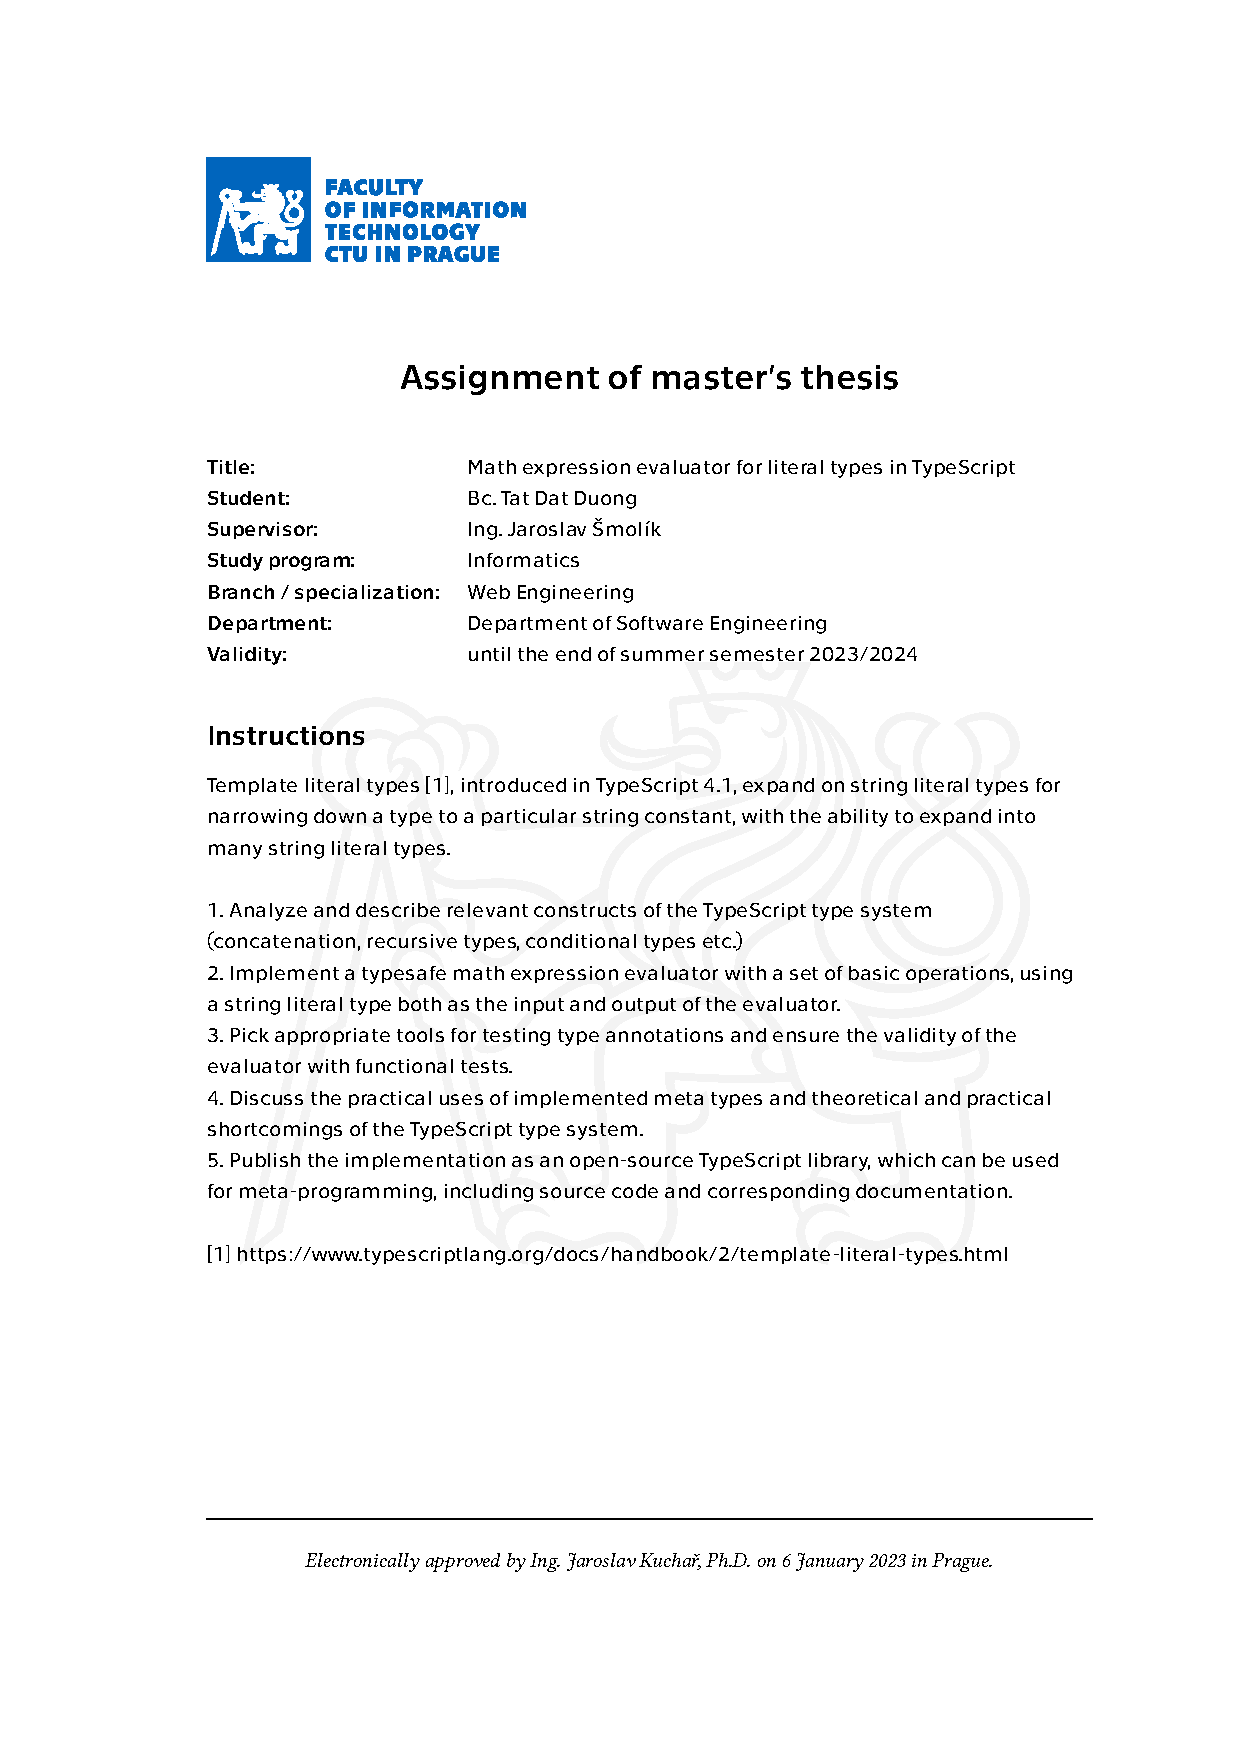
\includepdf{assignment-include.pdf} % replace that file with your thesis assignment provided by study office

\thispagestyle{empty}\cleardoublepage\maketitle % do not remove these three commands

\imprintpage % do not remove this command

\tableofcontents % do not remove this command
%%%%%%%%%%%%%%%%%%%%%%
% list of other contents: figures, tables, code listings, algorithms, etc.
% add/remove commands accordingly
%%%%%%%%%%%%%%%%%%%%%%
\listoffigures % list of figures
\begingroup
\let\clearpage\relax
\listoftables % list of tables
% \lstlistoflistings % list of source code listings generated by the listings package
\listoflistings % list of source code listings generated by the minted package
\endgroup
%%%%%%%%%%%%%%%%%%%%%%
% list of other contents END
%%%%%%%%%%%%%%%%%%%%%%

%%%%%%%%%%%%%%%%%%%
% ACKNOWLEDGMENT
% FILL IN / MODIFY
% This is a place to thank people for helping you. It is common to thank your supervisor.
%%%%%%%%%%%%%%%%%%%
\begin{acknowledgmentpage}
  Chtěl bych poděkovat především sit amet, consectetuer adipiscing elit. Curabitur sagittis hendrerit ante. Class aptent taciti sociosqu ad litora torquent per conubia nostra, per inceptos hymenaeos. Cras pede libero, dapibus nec, pretium sit amet, tempor quis. Sed vel lectus. Donec odio tempus molestie, porttitor ut, iaculis quis, sem. Suspendisse sagittis ultrices augue.
\end{acknowledgmentpage}
%%%%%%%%%%%%%%%%%%%
% ACKNOWLEDGMENT END
%%%%%%%%%%%%%%%%%%%

%%%%%%%%%%%%%%%%%%%
% DECLARATION
% FILL IN / MODIFY
%%%%%%%%%%%%%%%%%%%
% INSTRUCTIONS
% ENG: choose one of approved texts of the declaration. DO NOT CREATE YOUR OWN. Find the approved texts at https://courses.fit.cvut.cz/SFE/download/index.html#_documents (document Declaration for FT in English)
% CZE/SLO: Vyberte jedno z fakultou schvalenych prohlaseni. NEVKLADEJTE VLASTNI TEXT. Schvalena prohlaseni najdete zde: https://courses.fit.cvut.cz/SZZ/dokumenty/index.html#_dokumenty (prohlášení do ZP)
\begin{declarationpage}
  I hereby declare that the presented thesis is my own work and that I have cited all sources of information in accordance with the Guideline for adhering to ethical principles when elaborating an academic final thesis.

  I acknowledge that my thesis is subject to the rights and obligations stipulated by the Act No. 121/2000 Coll., the Copyright Act, as amended. In accordance with Article 46(6) of the Act, I hereby grant a nonexclusive authorization (license) to utilize this thesis, including any and all computer programs incorporated therein or attached thereto and all corresponding documentation (hereinafter collectively referred to as the “Work”), to any and all persons that wish to utilize the Work. Such persons are entitled to use the Work in any way (including for-profit purposes) that does not detract from its value. This authorization is not limited in terms of time, location and quantity.
\end{declarationpage}
%%%%%%%%%%%%%%%%%%%
% DECLARATION END
%%%%%%%%%%%%%%%%%%%

\printabstractpage % do not remove this command

%%%%%%%%%%%%%%%%%%%
% SUMMARY
% FILL IN / MODIFY
% OR REMOVE ENTIRELY (upon agreement with your supervisor)
% (appropriate to remove in most theses)
%%%%%%%%%%%%%%%%%%%
\begin{summarypage}
  \section*{Summary section}

  \lipsum[1][1-8]

  \section*{Summary section}

  \lipsum[2][1-6]

  \section*{Summary section}

  \lipsum[3]

  \section*{Summary section}

  \lipsum[2]

  \section*{Summary section}

  \lipsum[1][1-8] Lorem lorem lorem.
\end{summarypage}
%%%%%%%%%%%%%%%%%%%
% SUMMARY END
%%%%%%%%%%%%%%%%%%%

%%%%%%%%%%%%%%%%%%%
% ABBREVIATIONS
% FILL IN / MODIFY
% OR REMOVE ENTIRELY
% List the abbreviations in lexicography order.
%%%%%%%%%%%%%%%%%%%
\printglossaries

%%%%%%%%%%%%%%%%%%%
% ABBREVIATIONS END
%%%%%%%%%%%%%%%%%%%

\mainmatter\mainmatterinit % do not remove these two commands

%%%%%%%%%%%%%%%%%%%
% THE THESIS
% MODIFY ANYTHING BELOW THIS LINE
%%%%%%%%%%%%%%%%%%%

\setcounter{page}{1}

\chapter{Introduction}
% \chapter*{Introduction}\addcontentsline{toc}{chapter}{Introduction}\markboth{Introduction}{Introduction}

\section{Motivation}

\section{What is static type system}

In statically typed languages, a data type of a variable is known at compile time. The compiler uses the additional information about data types to verify the source code during compilation. The data type itself can be deduced from the usage in the code (type inferrence) or a programmer explicitly specifies the data type of a variable before usage. Example of such languages using static typing are for instance Java, C\#, C++, etc.

Whereas in dynamically typed languages, the type of a variable is determined at runtime based on the value being assigned. This flexibility allows developers to write code faster in exchange of raised likelihood of type relared errors in runtime. Example of such languages are Python, Ruby, PHP and most notably JavaScript.

Static typing offers numerous compelling benefits, that can enhance the development process:
\begin{itemize}
  \item Reduced likelihood of errors
  \item Self-documenting
  \item Less code to capture intent
  \item More confidence when refactoring
  \item Better tooling
\end{itemize}

First, with static typing a large class of errors are caught much earlier in the development process, thereby reducing the likelihood of bugs and runtime issues, which are inherently harder to catch and debug.

Even though developers might need to write more code to specify the types for the variable, if code is properly structured, the type system is able to determine the intent of the developer without writing additional code.



Additionally, with writing types, developers are actively self-documenting the code, which in turn increases the readability of the code, making the codebase easier to maintain and understand. Refactoring is also significantly easier with static types, as potential errors are raised during compile time instead of runtime.


\section{Cool stuff being done with TS}


\chapter{Analysis}

\section{Static Typing in JavaScript}

JavaScript is a dynamically typed programming language where users do not need to assign types to a variable or a function. The type is automatically inferred by the JavaScript engine at runtime. This feature lowers the barrier of entry to writing JavaScript code, allowing developers to prototype and write code quickly. It can plausibly be one of the possible growth drivers of JavaScript in the last decade, making it the most commonly used programming language, according to the 2022 Stack Overflow Developer Survey \cite{StackOverflowDeveloper}.

However, dynamic typing has its drawbacks. It is harder to detect trivial errors in the code without running it beforehand, and it is more difficult to refactor the code without breaking it, which often leads to poor software quality \cite{schumacherConceptsProgrammingLanguages2015}. Proponents of static typing insist that static types allow developers to spot potential bugs and mistakes earlier during development and that static typing allows for better tooling, such as richer code completion and better refactoring tools.

There is an upcoming \acrshort{tc39} proposal for adding type annotations in JavaScript, broadly inspired by the TypeScript syntax \cite{ECMAScriptProposalType2023}. These annotations are only useful for build-time tooling as they are ignored in runtime. The proposal suggests that these annotations should be erased by an additional compilation step. Even though users can already provide static types using JSDoc right now, the syntax is not as clean as the proposed TypeScript-like syntax.

Regardless, many projects aim to introduce static typing to JavaScript, such as Flow or TypeScript, or alternative languages which compile back to JavaScript, such as Elm or ReScript.

\subsection{Elm}

Elm is a functional programming language designed specifically for building web applications \cite{ElmDelightfulLanguage}. The language compiles to JavaScript and has a strong static Hindley-Milner-based type system, which allows inferring types more often and reliably. Elm does not provide any escape hatches, such as \code{any} in TypeScript. Thus it is harder to write unsafe code, as the types must be valid for the code to be successfully compiled.

Elm also includes a lot of quality-of-life improvements and benefits, for instance: enforced purity of functions, out-of-the-box immutability, \code{case} pattern matching, JSON decoders and encoders for strict parsing, \code{Maybe} and \code{Result} monads for avoiding \code{null} and \code{undefined} references or its own virtual DOM implementation for efficient rendering of interactive user interfaces. Notably, the Elm Architecture, where the application code is organised into three parts: model, update and view \cite{ElmArchitectureIntroduction}, has greatly inspired other libraries and frameworks such as Redux \cite{PriorArtRedux2022}.

\subsection{ReScript}

ReScript is a programming language built on top of the OCaml toolchain. Unlike Flow or TypeScript, ReScript is not a superset of JavaScript. Instead, the language compiles into JavaScript. ReScript was created as a spin-off from the Reason programming language and accompanying BuckleScript compiler, aiming to vertically integrate and streamline the adoption barrier caused by the need to be familiar with multiple unrelated tools and toolchains \cite{BuckleScriptReasonRebranding}.

The language aims to be more sound with more powerful type inference than TypeScript, borrowing the Hindler-Milner type system from OCaml implementation \cite{EfficientInsightfulGeneralization, HistoryReScript2022}. Thus, most of the time, the types can be automatically inferred without annotating them explicitly, whereas TypeScript utilises bidirectional type-checking \cite{ReconstructingTypeScriptPart}.

\subsection{Flow}

Flow is a static type checker for JavaScript \cite{chaudhuriFastPreciseType2017, Flow2023}, which allows developers to annotate their code with static types. Flow is developed by Meta and is internally used in production by Facebook, Instagram and React Native. Type annotations in Flow are fully erasable, meaning that the type annotations are fully removed from the Flow code in order to emit valid JavaScript code. The checking of these types occurs at compile-time before removal in build-time. Flow is also a superset of JavaScript, which means any JavaScript code is a valid Flow code.

One of the primary goals of Flow is to provide type soundness, the ability to catch every error that might happen in runtime at compile-time, no matter how likely it is to happen. A valid Flow code can provide developers with some guarantees about the type a value has in runtime, at the expense of catching errors that are unlikely to happen in runtime.

Both Flow and TypeScript are similar regarding features as of the time of writing. Most of the type-safety differences between Flow and TypeScript have been addressed with the newer versions of TypeScript, even though a \say{provably correct} type system is a specific non-goal of the TypeScript team \cite{TypeScriptDesignGoals}. However, developers must opt-in to these features by setting \code{"strict"} to \code{"true"} in \code{tsconfig.json}, whereas these features are enabled by default in Flow.

\subsection{TypeScript}

TypeScript is a statically typed programming language developed and maintained by Microsoft \cite{TypeScriptJavaScriptSyntax}. It is a language that transpiles into JavaScript and adds static type-checking to JavaScript \cite{DocumentationTypeScriptJavaScript}. Unlike Elm or ReScript, TypeScript is a syntactical superset of JavaScript, which means that any valid JavaScript code can be a valid TypeScript code\footnote{With a lax type checker configuration}. Similar to Flow, type annotations provided by the developer are fully erasable either by the TypeScript compiler \acrshort{cli} or by other community build tools, such as \code{babel}\cite{BabelBabel2023}, \code{esbuild}\cite{EsbuildExtremelyFast} or \code{swc}\cite{SWCRustbasedPlatform}.

Type system in TypeScript is considered to be less sound and more forgiving, as soundness is stated as an explicit non-goal of the design team of TypeScript \cite{TypeScriptDesignGoals}, with emphasis on striking a balance between productivity and correctness. By default, the TypeScript type checker is not strict, and the language itself includes an escape hatch for developers to opt out of type-checking by using the \code{any} type or using \code{@ts-ignore} comment annotations. Nevertheless, with proper type checker configuration, the type system of TypeScript can be as sound as in Flow.

Both Flow and TypeScript support advanced features such as generics and utility types, with the latter supporting template string literal types and better support for conditional types, unlocking the potential of writing more expressive types, which this master thesis will further explore in more detail.

With deep integration with Visual Studio Code \cite{VisualStudioCode}, the rich build ecosystem and high compatibility with existing JavaScript libraries and tools, TypeScript has become one of the fastest growing languages in terms of usage according to the 2022 Octoverse report by Github \cite{Octoverse2022State}.


\section{Usage of TypeScript}

The TypeScript project is made of two major parts available to developers:

\begin{itemize}
  \item \code{tsc}: the TypeScript Compiler, which is responsible for both type checking and outputting valid JavaScript files,
  \item \code{tsserver}: the TypeScript Standalone Server, which encapsulates the TypeScript Compiler and language services for use in editors and \acrshort{ide}s \cite{StandaloneServerTsserver}.
\end{itemize}

While a type-checker is most likely executed manually more often and is the entry point for developers when using TypeScript, the language server is equally as useful, as it communicates with the editor via \acrfull{lsp} to provide important language services. These include code completion, auto-importing, symbol renaming etc.

Unlike in the other languages, the compilation step itself is understood to only mean the type erasure itself. Even though the source code itself can have various type errors, \code{tsc} will still, by default, emit JavaScript files as long as the input source file can be parsed by both the scanner and the parser. This allows developers to progressively update their code and iterate quickly on the functionality without immediately dealing with the type errors, acting more as a linter than a compiler. Regardless, in this thesis, \say{compiling} and \say{type-checking} will be used interchangeably.


\section{Typescript syntax}

In TypeScript, types are generally annotated using \code{:[type annotation]} syntax, which introduces annotations to various JavaScript constructs, including variables, function parameters and function return values, to add constraints to values. Type annotations in TypeScript can be classified into multiple categories, such as primitive types, literal types, data structure types, union types and intersection types. The subsequent sections will provide a comprehensive exploration of these types alongside more advanced types, such as conditional, mapped, and recursive types. A basic example of TypeScript type annotation is presented in Listing \ref{lst:basic-annotation}.

\begin{listing}[ht]
  \begin{minted}{TypeScript}
const prefix: string = "Hello world"
const user: {
  name: string;
  age: number
}

function formatUserGreeting(
  user: {
    name: string;
    age: number;
  }, 
  message: string
): string {
  return [message, user.name].join(" ");
}

const greeting: string = formatUserGreeting(user, prefix); 
\end{minted}
  \caption{Basic TypeScript annotation example}\label{lst:basic-annotation}
\end{listing}

At runtime, every variable has a single concrete value, but in TypeScript, the variable is represented solely by its type. A useful mental model for understanding types is to think of the type as a set of permitted values \cite{vanderkamEffectiveTypeScript622019}, effectively constituting the domain of the type.

Developers have the ability to declare types directly in type annotations, but in certain cases, there may be a need to reuse the same type in multiple annotations. In order to avoid excessive repetition of the same declaration, type aliases can be employed to refer to a type by a name. These type variables act as an alias, which can be used in place of the type itself. The Listing \ref{lst:type-aliases} shows a refactored \code{formatUserGreeting} function of the previous Listing \ref{lst:basic-annotation} using type aliases.

\begin{listing}[ht]
  \begin{minted}{TypeScript}
type User = {
  name: string;
  age: number
}

const prefix: string = "Hello world"
const user: User

function formatUserGreeting(
  user: User, 
  message: string
): string {
  return [message, user.name].join(" ");
}
\end{minted}
  \caption{Type aliases}\label{lst:type-aliases}
\end{listing}

\subsection{Primitive Types}

A primitive value refers to data that is neither an object nor possesses methods or properties. These primitive values are immutable, which means they cannot be altered. The TypeScript type system provides a comprehensive representation of these primitives, as seen in Listing \ref{lst:primitive-types} describing the following primitive types:

\begin{listing}[ht]
  \begin{minted}{TypeScript}
type StringPrimitive = string
type NumberPrimitive = number
type BigintPrimitive = bigint
type BooleanPrimitive = boolean
type UndefinedPrimitive = undefined
type NullPrimitive = null
type SymbolPrimitive = symbol
\end{minted}
  \caption{Primitive Types}\label{lst:primitive-types}
\end{listing}

Certain primitive types represent a singular data value, such as \code{null} or \code{undefined}, but many of these primitives can represent multiple values (\code{boolean} can represent either \code{true} or \code{false}), or even an infinite range of values, as observed in the case of \code{number}, \code{bignumber} or \code{string} type.

\subsection{Literal Types}

Literal types are used to describe an exact value as a type. From the point of view of the type system, a literal type is a subset of one of the following primitive types: \code{string}, \code{number}, \code{bignumber} or \code{boolean}\footnote{Both \code{null} and \code{undefined} are literal types as well}, as seen in Listing \ref{lst:literal-types}\footnote{The following listing uses union types, described in Section \ref{sec:union-intersection}}.

\begin{listing}[ht]
  \begin{minted}{TypeScript}
type Literal = "foo" | 42 | true | 100n;

// Valid code
const Valid: Literal = "foo"

// @ts-expect-error Type '"bar"' is not assignable to type 'Literal'
const Invalid: Literal = "bar" 
\end{minted}
  \caption{Literal Types}\label{lst:literal-types}
\end{listing}

\subsection{Types for data structures}\label{sec:typescript-data-structures}

TypeScript also allows annotating data structures such as objects and arrays with four possible types, depending on the enumerability of items and their types. The syntax overview can be seen here in Listing \ref{lst:data-structures}.

\begin{itemize}
  \item \code{tuple} type for describing an array with a fixed number of elements, possibly with a different type for each element,
  \item \code{array} type for describing an array with an unknown length, and the values are of the same type,
  \item \code{record} type for describing an object with an unknown number of keys, and the values are of the same type,
  \item \code{object} type or an \code{interface} for describing an object with a finite set of keys with values of different types per key.
\end{itemize}

\begin{listing}[ht]
  \begin{minted}{TypeScript}
interface ObjectStructure {
  foo: string;
  bar: number;
}

type ObjectStructure =  
  | { foo: string, bar: number }

type RecordStructure 
  | { [key: string]: number }
  | Record<string, number>

type TupleStructure = [number, string]

type ArrayStructure = number[]
\end{minted}
  \caption{Data structures}\label{lst:data-structures}
\end{listing}

TypeScript syntax offers two notations which can be used for describing objects with a finite set of key-value pairs in TypeScript: \code{object} and \code{interface}. There are some key differences between these two notations:

\begin{enumerate}
  \item The \code{object} type uses the type alias syntax, whereas an interface is defined using a special \code{interface} keyword.
  \item TypeScript allows multiple declarations of \code{interface} later merged during interpretation. This can be especially useful when augmenting non-TypeScript modules \cite{DocumentationDeclarationMerging}.
  \item Even though both support object merging, \code{interface} can be implemented by classes, ensuring that the class adheres to the structure defined by the interface. \code{object} types cannot be directly implemented by a class.
  \item Merging \code{interface} declarations is more performant when merging multiple declarations than an intersection of \code{object} types \cite{Performance}.
\end{enumerate}

TypeScript uses structured typing, which entails that TypeScript only validates the shape of the data. In essence, if the shape of the data is consistent with that of the type, it is considered to be of that type, as seen in Listing \ref{lst:structured-typing}. This concept is commonly referred to as duck typing, essentially: \say{If it walks like a duck and quacks like a duck, it is a duck.}

\begin{listing}[ht]
  \begin{minted}{TypeScript}
type DuckLike = { quack: () => void; type: string };

const Duck: DuckLike = {
  quack: () => console.log("duck!"),
  type: "duck",
};

// This will be still valid
const Goose: DuckLike = {
  quack: () => console.log("goose!"),
  type: "goose",
};
\end{minted}
  \caption{Structured typing}\label{lst:structured-typing}
\end{listing}

However, there are real-world use cases for a nominal type system, where two variables are distinguished by their type name, despite having the same shape. Emulating nominal typing in TypeScript can be achieved by introducing an unused property in order to break structural compatibility \cite{NominalTyping}, as demonstrated in Listing \ref{lst:nominal-types-emulation}.

\begin{listing}[ht]
  \begin{minted}{TypeScript}
type DuckLike = { quack: () => void; type: "duck" };

const Duck: DuckLike = {
  quack: () => console.log("duck!"),
  type: "duck",
};

// This will not be valid
const Goose: DuckLike = {
  quack: () => console.log("goose!"),
  type: "goose",
};
\end{minted}
  \caption{Nominal typing in TypeScript}\label{lst:nominal-types-emulation}
\end{listing}

\subsection{Union and intersection types}\label{sec:union-intersection}

Revisiting the concept of types as sets of values, as seen in Listing \ref{lst:literal-types}, assigning a value disallowed by the literal type will result in a type error. In TypeScript, a type is considered \say{assignable} if it is either a \say{member of} the set of permitted values defined by the type (when describing relationships between a value and a type) or a \say{subset of} the sets (when describing relationships between two types).

When there is a requirement to describe a type that encompasses multiple types, combining two sets of permitted values into a single set, union types can be utilised. Union types are defined by the union operator represented by the \code{|} symbol, separating the types that are being combined, referred to as \say{union members} \cite{DocumentationEverydayTypes}. Essentially, \code{X | Y} can be read as a type for a value that can either be of type \code{X} or \code{Y}.

Since a union type can contain a value from any of the member types, TypeScript permits only those operations that are valid for all member types within the union. If an operation is only valid for some of the union member types, type narrowing must be performed. Type narrowing is a process of refining a broader type to a more specific narrow one, capturing a subset of values of the original broader type.

An example of type narrowing can be seen in Listing \ref{lst:union-types}, where the function \code{printUserId} can accept both a \code{string} or a \code{number} as an argument. In order to invoke \code{toUpperCase()}, a method valid only for values of \code{string} type, it is necessary to perform a check if the parameter is a \code{string}. Afterwards, TypeScript has the necessary information to infer that the type of the checked value must be necessary a \code{string} and permits the invocation of \code{toUpperCase()}.

\begin{listing}[ht]
  \begin{minted}{TypeScript}
function printUserId(id: string | number) {
  if (typeof id === "string") {
    return id.toUpperCase()
  } else {
    return id
  }
}
  \end{minted}
  \caption{Union types with simple narrowing}\label{lst:union-types}
\end{listing}

An intersection of types can be represented by the \code{\&} operator. Similarly to the union type, \code{X \& Y} can be read as a type for a value that can simultaneously belong to type \code{X} and \code{Y}. Intersection types are particularly relevant when working with object types, as an intersection of two object types has all properties of both object types. The rationale is that an object with merged properties is assignable to all of the intersection member types. For this particular reason, intersection types are commonly used to merge multiple object types, as seen in \ref{lst:intersection-types}\footnote{It is also possible to use the \code{extends} keyword to merge interfaces instead}.

\begin{listing}[ht]
  \begin{minted}{TypeScript}
type Intersection = { a: string } & { b: number }
const item: Intersection = { a: "a", b: 1 }
  \end{minted}
  \caption{Intersection types}\label{lst:intersection-types}
\end{listing}

\subsection{\code{keyof} type and indexed access types}

The indexed access type is used to access a specific property type of a record or a tuple type. The syntax of indexed access types mirrors the syntax for accessing an object in JavaScript, as seen in Listing \ref{lst:indexed-access-types}. It is also possible to use unions as keys to get types of multiple properties of an object type.

\begin{listing}[ht]
  \begin{minted}{TypeScript}
type User = { firstName: string; lastName: string; age: number }

type Age = User["age"] 
type Names = User["firstName" | "lastName"]
\end{minted}
  \caption{Indexed access types}\label{lst:indexed-access-types}
\end{listing}

The \code{keyof} keyword operator can be used to get all possible keys of an object type. This will return an union of all keys of the provided data structure type. These are especially useful when working with mapped types later on. An example can be seen in Listing \ref{lst:keyof}.

\begin{listing}[ht]
  \begin{minted}{TypeScript}
type User = { firstName: string; lastName: string; age: number }
type Keys = keyof User
//   ^? "firstName" | "lastName" | "age"
\end{minted}
  \caption{Usage of \code{keyof}}\label{lst:keyof}
\end{listing}

\subsection{Special data types}

When working with unions and intersections, it is often necessary to be able to describe a type, which can describe a union of all possible types or a type created by intersecting two types with no related properties. These types are referred to as universal supertypes and universal subtypes, respectively. Universal supertypes, also known as top types, are types that are a superset of all other types and are used to represent any possible value. Whereas universal subtypes, also known as bottom types, are types that are a subset of all other types and are often used to describe a type that has no permitted values.

TypeScript includes two top universal supertypes: \code{any} and \code{unknown}. In the case of \code{any}, every type is assignable to type \code{any} and type \code{any} is assignable to every type \cite{TopTypesAny}. In general, \code{any} can be used as an escape hatch to opt out of type checking. This does have unintended consequences, as \code{any} is assignable to every type; it can be assigned to a different type without any warnings. This is especially problematic when dealing with external data as the return type of \code{JSON.parse()} is \code{any}. An example of assignability can be seen at Listing \ref{lst:any-assignability}.

\begin{listing}[ht]
  \begin{minted}{TypeScript}
let data: any = JSON.parse("...") 

// All of these are valid TypeScript code
data = null
data = true
data = {}

// Still valid code, opting out of type checking
const a: null = data
const b: boolean = data
const c: object = data
  \end{minted}
  \caption{Assignability of any}\label{lst:any-assignability}
\end{listing}

\code{unknown} acts as a more restrictive version of \code{any}. Every type is assignable to type \code{unknown}, but \code{unknown} is not assignable to any other type, which can be seen at Listing \ref{lst:unknown-assignability}. In order to assign \code{unknown} to a different type, type narrowing must be performed by either using type guards, type assertions, equality checks or other assertion functions.

\begin{listing}[ht]
  \begin{minted}{TypeScript}
let data: unknown = JSON.parse("...") 

// All of these are valid TypeScript code
data = null
data = true
data = {}

// Not valid, as unknown is not assignable to any other type
const a: null = data
const b: boolean = data
const c: object = data
  \end{minted}
  \caption{Assignability of unknown}\label{lst:unknown-assignability}
\end{listing}

Finally, \code{never} is a bottom type, acting as a subtype of all other types, representing a value that should never occur. In the context of the theory of mathematical logic, \code{never} acts as a logical contradiction, describing a value that may never exist. No other type can be assigned to \code{never} nor \code{never} cannot be assigned to any other type. \code{never} can be found when attempting to intersect two types that have no properties in common, such as \code{string \& number}.

\code{void} is a specific type used to signify a function which does not return a value. There is a notable difference between the usage of \code{void} when used in context, describing a type for a function with \code{void} return type, and when used in the function declaration, as seen in Listing \ref{lst:void-return-type}. The former is used to describe a situation when an implementation of a \say{void function} does return a value but should be ignored. The latter does enforce that a function should not return a value at all.

\begin{listing}[ht]
  \begin{minted}{TypeScript}
type voidFn = () => void

// Valid code
const fn1: voidFn = () => true

function fn2(): void {
  // @ts-expect-error Not valid, as void functions cannot return a value
  return true
}
\end{minted}
  \caption{Return type void}\label{lst:void-return-type}
\end{listing}

\subsection{Enumerations}

\code{enum} type is a distinct subtype used to describe a set of named constants. Instead of using individual variables for each constant, an \code{enum} provides an organised way to express a collection of related values. \code{enum} is one of the few TypeScript features which introduce an additional code added to the compiler output, and enums refer to real objects at runtime.

An \code{enum} type consists of members and their corresponding initialisers for the runtime value of the member. There are two types of enums in TypeScript: numeric enums and string-based enums. In numeric enums, each member is assigned a numeric value, as seen in Listing \ref{lst:numeric-enums}. Each member can have an optional initialiser to specify an exact number corresponding to a member. If omitted, the value of the member will be generated by auto-incrementing from previous members.

\begin{listing}[ht]
  \begin{minted}{TypeScript}
enum Direction {
  Up = 1,
  Down,
  Left,
  Right,
}
\end{minted}
  \caption{Numeric enums}\label{lst:numeric-enums}
\end{listing}

String-based enums are similar in nature, where each member is assigned a string value instead. Each member thus must have an initialiser with a string literal, as seen in Listing \ref{lst:string-based-enums}. The key benefit of string-based enums is that they tend to keep their semantic value well when serialising, which is especially helpful when debugging, as the values of numeric enums tend to be opaque.

\begin{listing}[ht]
  \begin{minted}{TypeScript}
enum Direction {
  Up = "UP",
  Down = "DOWN",
  Left = "LEFT",
  Right = "RIGHT",
}
\end{minted}
  \caption{String-based enums}\label{lst:string-based-enums}
\end{listing}

\subsection{Namespaces}

In TypeScript, namespaces, formally known as internal modules, are used to organise code and prevent naming conflicts in the global scope. In order to create a namespace, the \code{namespace} keyword is used, followed by the identifier of the namespace. The code within the namespace, also called the scope of the namespace, is isolated from the global environment, as seen in Listing \ref{lst:namespace}. Only constructs explicitly marked as exported are accessible outside of the namespace, exposed as a single variable with the name of the namespace.

\begin{listing}[ht]
  \begin{minted}{TypeScript}
namespace Example {
  type Foo = "Foo"
  const foo: Foo = "Foo"
  
  export type Bar = "Bar"
  export const bar: Bar = "Bar"
}

// @ts-expect-error Not accessible
const a = Example.foo 

// Valid code
const b = Example.bar
\end{minted}
  \caption{Namespace usage}\label{lst:namespace}
\end{listing}

One key benefit of namespaces is the ability to merge multiple namespaces across files. As long as the name of multiple namespaces is the same, the declarations will be merged into a single declaration. This feature can split large scopes into multiple files while exposing all of the properties as a single variable.

\subsection{Generic Types}

In many cases, it is necessary to write sufficiently reusable code that must function with types not known beforehand. Generic types allow the development of such reusable components that can work over a variety of types rather than a single one. Generic types are created by defining a type parameter that can be used as a placeholder for a specific type. The consumers can then replace the placeholder with their desired types when using the component. In TypeScript, generic types can be defined on interfaces, functions and classes.

To illustrate the point, consider the implementation of the built-in \code{Array} type found in the \code{lib.*.d.ts} files (a subset can be seen at Listing \ref{lst:array-type}). The \code{Array<T>} is a generic type, which accepts a single type argument \code{T} and is used to describe the type of the elements in the array. The type argument \code{T} is later used both in arguments and return types of the methods of the \code{Array<T>} type: \code{push()} accepts only elements of the same type as the array while \code{pop()} will return an element of the same type.

\begin{listing}[ht]
  \begin{minted}{TypeScript}
interface Array<T> {
  push(...items: T[]): number;

  pop(): T | undedfined;
}

const strArr: Array<string> = []
const numArr: Array<number> = []

strArr.push("one", "two")
numArr.push(1, 2)

const a = strArr.pop()
//    ^? string

const b = numArr.pop()
//    ^? number
\end{minted}
  \caption{Array type}\label{lst:array-type}
\end{listing}

Generic types can be interpreted as functions in a meta-programming language found inside the TypeScript type system itself. The meta-programming language implements some of the key concepts found in the functional programming paradigm.

Generic types are considered first-class citizens in the language, being able to be passed as arguments into other generic types, similar to functions in a functional programming language. Generic types are also pure and cannot have any side effects during type checking. Recursion is also used in the meta-programming language to break down complex problems into smaller ones and solve them independently.

There is a notable omission, however: generic types cannot receive other generic types as type arguments \cite{TypeInferenceHigherorder}. Thus, higher-order functions are not permitted \footnote{There is a way to create such type using HOTScript, more on that later}.

\subsection{Type constraints with \code{extends}}

When writing generic types, it is essential to describe some expectations that a type argument must satisfy. For example, it may be necessary to accept types which do have a certain property, such as \code{length} as seen in Listing \ref{lst:extends}. To achieve this, the \code{extends} keyword can be used to describe the constraints of the type.

\begin{listing}[ht]
  \begin{minted}{TypeScript}

function getLength<T extends HasLength>(obj: T): number {
  return obj.length
}

const a = getLength("hello")
const b = getLength([1, 2, 3])
const c = getLength({ length: 10 })

// @ts-expect-error 
// Argument of type '{ foo: string; }' is not 
// assignable to parameter of type 'HasLength'.
const d = getLength({ foo: "bar" })
\end{minted}
  \caption{Type constraints with \code{extends}}\label{lst:extends}
\end{listing}


As intended, the generic function will no longer accept arbitrary types. Instead, only types that satisfy the imposed constraints can be passed to the function as the argument.

\subsection{Conditional types}

Within the TypeScript meta-language, developers can write conditions and branching logic using conditional types. Conditional types follow a syntax similar to the conditional ternary operators with another case of overloading the \code{extends} keyword: \code{Input extends Expect ? A : B}. This can be read as \say{If type Input is assignable to type Exepct, then the type resolves to type A, otherwise to type B.} An example can be seen in Listing \ref{lst:conditional-types}, where the \code{IsString<T>} type will resolve to \code{true} if the type argument \code{T} is assignable to \code{string} and to \code{false} otherwise.

\begin{listing}[ht]
  \begin{minted}{TypeScript}
type IsString<T> = T extends string ? true : false
\end{minted}
  \caption{Conditional types}\label{lst:conditional-types}
\end{listing}

The \code{infer} keyword can be used to deduce or extract a specific type within the scope of conditional types, essentially acting as a way to perform pattern matching. With \code{infer}, a new generic type variable is introduced, which can be later used within the true branch of the conditional type, as seen in the implementation of the \code{ReturnType<T>} utility type in Listing \ref{lst:infer}. The \code{ReturnType<T>} type will resolve to the return type of the type argument \code{T}.

\begin{listing}[ht]
  \begin{minted}{TypeScript}
type ReturnType<T> = T extends (...args: any) => infer R ? R : never;
\end{minted}
  \caption{Infer in conditional types}\label{lst:infer}
\end{listing}

Since TypeScript version 4.7 \cite{AnnouncingTypeScript4.7}, an additional type constraint can be added for the inferred type, which will be checked before the conditional type is resolved. This method is useful when attempting to avoid an additional nested conditional type, as seen in Listing \ref{lst:infer-constraint}, where the aim is to return the first element of the tuple type only if it is a string.

\begin{listing}[ht]
  \begin{minted}{TypeScript}
type FirstIfString<T> =
  T extends [infer S extends string, ...unknown[]]
    ? S
    : never;

// is equivalent to 
type FirstIfString<T> =
  T extends [infer S, ...unknown[]]
    ? S extends string ? S : never
    : never;
\end{minted}
  \caption{Type constraints within infer}\label{lst:infer-constraint}
\end{listing}

When a union type is provided within the conditional type, the conditional type will be resolved for each member type in the union separately, effectively distributing the union type. In order to prevent such behaviour, the type argument can be wrapped in a tuple or any other structure type.

\begin{listing}[ht]
  \begin{minted}{TypeScript}
type ToArray<Type> = Type extends any ? Type[] : never;

// $ExpectType string[] | number[]
type A = ToArray<string | number> 

type ToArrayNonDist<Type> = [Type] extends [any] ? Type[] : never;

// $ExpectType (string | number)[]
type B = ToArrayNonDist<string | number> 
\end{minted}
  \caption{Distributing union types}\label{lst:distribute}
\end{listing}

\subsection{Mapped types}

Occasionally, it is necessary to transform a type into another type. For instance, a new type may need to be created that is a copy of the original type but with all properties marked as optional. This can be accomplished with mapped types. Mapped types are types which are created using the syntax for index signatures, commonly used in JavaScript for properties not declared ahead of time. An example is shown in Listing \ref{lst:mapped-types}, where the generic type \code{ToBoolean<T>} will create a new type which will take all properties from \code{T} and change their values to \code{boolean}.

Mapping modifiers can also be specified to affect the mutability or optionality of a property: \code{readonly} and \code{?} respectively. Prefixing the modifier with either \code{+} or \code{-} will either add or remove the modifier to the property\footnote{+ is assumed by default if omitted}. This can be seen in the \code{Optional<T>} type in Listing \ref{lst:mapped-types}, which will create a new type, which is a copy of the original type, but with all properties being optional.

\begin{listing}[ht]
  \begin{minted}{TypeScript}
type ToBoolean<T> = {
  [K in keyof T]: boolean
}

type Optional<T> = {
  [K in keyof T]+?: T[K]
}
\end{minted}
  \caption{Mapped types}\label{lst:mapped-types}
\end{listing}

Introduced in TypeScript 4.1 \cite{AnnouncingTypeScript4.1}, the \code{as} keyword can be used to re-map keys in mapped types, allowing developers to create, transform or filter out keys when creating a new type. An example is shown in Listing \ref{lst:mapped-as}, where the \code{Omit<T, Key>} creates a new object type based on type \code{T} with omitted properties which are assignable to \code{Key}.

\begin{listing}[ht]
  \begin{minted}{TypeScript}
type Omit<T, Key> = {
  [K in keyof T as Exclude<K, Key>]: T[K]
}
\end{minted}
  \caption{Using as in mapped types}\label{lst:mapped-as}
\end{listing}

\subsection{Recursive Types}

A recursive data type is a data type that includes a reference to itself within the type definition. Recursive types are useful for modelling complex or hierarchical data structures, such as linked lists or trees.

An example can be seen in Listing \ref{lst:recursive-types}, where the \code{Tree<Value>} generic type represents an object with a value of type \code{Value} and optional left and right subtrees of the same type.

\begin{listing}[ht]
  \begin{minted}{TypeScript}
type Tree<Value> = {
  value: Value,
  left?: Tree<Value>,
  right?: Tree<Value>
}
\end{minted}
  \caption{Modeling a binary tree with recursive types}\label{lst:recursive-types}
\end{listing}

By combining recursive types with generic types, typical recursive algorithms key for this thesis can be implemented in TypeScript. One such example can be seen at Listing \ref{lst:reduce-type}, where a \code{FromEntries<Entries>} generic type is implemented, converting a list of \code{[Key, Value]} tuples into a single object type.

First, an additional optional generic type parameter \code{Accumulator} is defined, with an initial type value of \code{{}}. For every tuple in a list, an object type containing the current key-value pair with \vcode{{ [K in Key]: Value }} is created and merged with the accumulator using the \vcode{&} operator. The merged object type is subsequently passed as the accumulator to the next iteration. Finally, the accumulator is returned when the list is empty, serving as the final object type.

\begin{listing}[ht]
  \begin{minted}{TypeScript}
type FromEntries<Entries, Accumulator = {}> =
  Entries extends [infer Entry, ...infer Rest]
    ? FromEntries<
        Rest,
        Entry extends [infer Key, infer Value]
          ? { [K in Key]: Value } & Accumulator
          : Accumulator
      >
    : Accumulator;
\end{minted}
  \caption{Reduce example}\label{lst:reduce-type}
\end{listing}

There are some limitations regarding recursive types. To prevent infinite recursion, TypeScript limits the instantiation depth to ensure a consistent and performant developer experience. As of writing, the limit is set to 100 levels for type aliases and 5 million type instantiations \cite{ImplementationCheckerTs2023}. Thanks to the tail-recursion elimination optimisation, the limit is set to 1000 levels for tail-optimized recursion types. Thus, it is desired to use tail recursion whenever possible.

Another limitation related to the generic recursive types is that the variables declared with \code{infer} do not inherit the constraints of the parent type, as seen in Listing \ref{lst:recursive-constraints}. As the \code{Tail} type lost the type constraint of \code{Haystack}, the tail cannot be passed as the new haystack of the \code{FilterWrong} type. Addressing this problem requires adding an extra type constraint to the inferred type.

\begin{listing}[ht]
  \begin{minted}{TypeScript}
type FilterWrong<Haystack extends string[], Needle extends string> =
  Haystack extends [infer Head, ...infer Tail]
    ? Head extends Needle
      // $ExpectError Type 'Tail' does not satisfy the constraint 'string[]'.
      ? [Head, ...FilterWrong<Tail, Needle>]
      : FilterWrong<Tail, Needle>
    : [];

type FilterCorrect<Haystack extends string[], Needle extends string> =
  Haystack extends [infer Head, ...infer Tail extends string[]]
    ? Head extends Needle
      ? [Head, ...FilterCorrect<Tail, Needle>]
      : FilterCorrect<Tail, Needle>
    : [];
\end{minted}
  \caption{Recursive types and type constraints}\label{lst:recursive-constraints}
\end{listing}

\subsection{Template Literal Types}

Finally, template literal types are based on the string literal types, allowing string interpolation and manipulation within the TypeScript type system. In the context of this thesis, template literal types are used to create a parser of mathematical expressions. However, template literal types can be utilised to create fully typed string-based \acrfull{dsl}.

Similar to the syntax of JavaScript template literal strings, backticks are used to create a new template literal type. When used with a string literal type, a template literal will create a new string literal type by concatenation \cite{DocumentationTemplateLiteral}. For example, the type \code{\`{}Hello \$\{"World"\}\`{}} will create a new string literal type \code{"Hello World"}.

Template literal types can be used with primitive types as well, the only limitation being that the primitive type must be stringifiable. That includes all of the primitive types except the \code{symbol} type. When created, these types are a subset of their primitive type and can be used to work as a validation mechanism matching a string of an expected format. For instance, the type \code{\`{}localhost:\$\{number\}\`{}} will create a new string literal type that will match a string of the format \code{localhost:PORT}, where \code{PORT} is a number.

The distributive nature of union types applies to template literal strings as well: the type will be applied for every member type of the union to the template literal, as seen in the Listing \ref{lst:union-template-literal}, where a new \code{Style} type is created with all of the possible combinations of the \code{Variants} and \code{Weights} types. Generally, avoiding combinations of big union types is preferable, as it can lead to worse type-checking performance or an error if a union type reaches 1\,000\,000 member types.

\begin{listing}[ht]
  \begin{minted}{TypeScript}
type Variants = "primary" | "secondary"
type Weights = 100 | 200 | 300

type Style = `${Variants}-${Weights}`
//   ^? | "primary-100" | "primary-200" | "primary-300" 
//      | "secondary-100" | "secondary-200" | "secondary-300"
\end{minted}
  \caption{Distributive nature of unions in template literal types}\label{lst:union-template-literal}
\end{listing}

Ultimately, inference in template literal types can be used to perform pattern matching within string literals with the combination of conditional types and the \code{infer} keyword. As shown in Listing \ref{lst:pattern-matching-template-literal}, a generic type \code{SplitString} is presented, which splits a literal string type into a tuple of substrings with a space as the delimiter. The aim is to perform pattern matching a string with \code{Head}, containing the first character, and \code{Rest}, including the rest of the split string, as the two inferred types as a result. Type constraints are also applied for the inferred types to ensure the types are assignable to \code{string}\footnote{Albeit unnecessarily, as TypeScript automatically applies the \code{string} type constraint in this instance}. Both of the inferred types are used to create a new tuple type, with \code{Head} being the first element of the tuple and \code{Rest} used in a recursive call to split the rest of the string.

\begin{listing}[ht]
  \begin{minted}{TypeScript}
type SplitString<Input extends string> = 
  Input extends `${infer Head extends string} ${infer Rest extends string}`
    ? [Head, ...SplitString<Rest>]
    : [Input];
\end{minted}
  \caption{Pattern matching with template literal types}\label{lst:pattern-matching-template-literal}
\end{listing}


\section{Prior Art}

There are multiple basic implementations of math operations in TypeScript. Tasks regarding basic math operations are even part of the TypeChallenges collection\cite{TypechallengesTypechallenges2023}. However, most of them only work on integers, as they work on tuple expansion, which will be further discussed in the implementation part of this thesis.

Nevertheless, multiple libraries in the \acrshort{npm} registry provide basic math calculations within the TypeScript type system, but none provide a fully typed parser of mathematical expressions. Some of the libraries found do provide type utilities that operate on floating-point numbers instead of integers, such as \code{type-fest} \cite{sorhusSindresorhusTypefest2023} or \code{typescript-lodash}\cite{kawayilinlinKawayiLinLinTypescriptlodash2023}. The most comprehensive implementation of math operations can be found in the \code{ts-arithmetic} library \cite{arielTypeLevelArithmetic2023}, which provides a fully typed implementation of division.

% \begin{itemize}
%   \item \code{kawayiLinLin/typescript-lodash} - floating point numbers, addition, subtraction, division by two
%   \item \code{arielhs/ts-arithmetic} - floating point numbers, addition, subtraction, multiplication, division, mod, negate, abs, compare, max, min, sign
%   \item \code{type-fest} - parsing float, sign modification
%   \item \code{hotscript} - integers, addition, subtraction, multiplication, division, mod, negate, abs, compare, max, min, sign
% \end{itemize}

\chapter{Implementation}

This chapter delves into the implementation of the mathematical expression evaluator using the TypeScript type system. The work being done in this thesis is realised into two major parts: implementing various mathematical operations and parsing and evaluating string literals containing a mathematical expression. The limitations and workarounds for TypeScript literal types are discussed, and by the end of this chapter, readers should gain a deeper understanding of the TypeScript type system when applied to non-trivial problem domains.

\section{Type representation of numbers}

As powerful as the type system in TypeScript is, there are certain limitations present when working with number literal types. Namely, although TypeScript type syntax does support representing specific numeric values through number literal types, these types do not directly support mathematical operations, such as addition or subtraction. Due to these limitations, other methods of representing numbers are explored for this thesis.

One approach to representing numbers in TypeScript is to use tuple types. As described in Section \ref{sec:typescript-data-structures}, tuple types allow developers to define a fixed-length JavaScript array where each element can have a specific type. As it represents a JavaScript array, the type includes all of the properties and methods found in an array, including the \code{length} property, which contains the actual number of elements in the tuple. This feature can be used to represent a number, as the length of the tuple can represent the number itself, as seen in Listing \ref{lst:tuple-representation}. The actual type of a member item in a tuple is irrelevant, as the implementation only cares about the length of the tuple, but for readability purposes, the literal type \code{0} can be used as the element type of a tuple.

\begin{listing}[ht]
  \begin{minted}{TypeScript}
type Zero = []
type Four = [0, 0, 0, 0] 

// $ExpectType 0
type ZeroValue = Zero['length']

// $ExpectType 4
type ZeroValue = Four['length']
\end{minted}
  \caption{Tuple representation of a number}\label{lst:tuple-representation}
\end{listing}

However, manually describing a tuple is tedious. Recursion can be employed to parse a number literal type to a tuple type, as seen in Listing \ref{lst:tuple-parse}. The \code{ParseNumber<Value>} generic type accepts a mandatory type argument \code{Value} that should be the length of the final tuple and an optional type argument \code{Acc} used to preserve the state of the recursion.

First, a check is performed to see if the length of \code{Acc} is equal to the \code{Value} by checking the assignability of types. If that is the case, the tuple type found in \code{Acc} is returned. Otherwise, the list is prepended with a new \code{0} element, and the generic type is instantiated recursively, until the length of \code{Acc} is assignable to \code{Value}.

\begin{listing}[ht]
  \begin{minted}{TypeScript}
type ParseNumber<
  Value extends number,
  Acc extends Array<0> = []
> = Acc["length"] extends Value ? Acc : ParseNumber<Value, [0, ...Acc]>
\end{minted}
  \caption{Parse a number literal type to a tuple type}\label{lst:tuple-parse}
\end{listing}

It is possible to reduce the number of recursions needed to create a tuple by expanding by digits instead of by increments of one. As seen in Listing \ref{lst:tuple-parse-digit}, where \code{ParsedNumber2} will first perform stringification of the number literal type \code{T} and infer the first digit recursively. The accumulator type parameter \code{Rest} is first expanded ten times by the \code{ExpandArrayTenTimes} generic type, and then the parsed digit is spread into \code{Rest} as well. The recursion is performed until the string found in \code{T} is empty, and the final \code{Rest} type is returned.

\begin{listing}[ht]
  \begin{minted}{TypeScript}

type ExpandArrayTenTimes<R extends Array<0>> = [
  ...R, ...R, ...R, ...R, ...R,
  ...R, ...R, ...R, ...R, ...R
]
    
type ParseNumber2<
  T extends number | string,
  Rest extends Array<0> = []
> = `${T}` extends `${infer Digit extends number}${infer R}`
  ? ParseNumber2<R, [...ExpandArrayTenTimes<Rest>, ...ParseNumber<Digit>]>
  : Rest
\end{minted}
  \caption{Parse by digit expansion}\label{lst:tuple-parse-digit}
\end{listing}

Even though this method of representing numbers is reasonably simple, it does come at a performance cost, as the length of the tuple must be equal to the represented number itself. As such, the checking time of the addition and subtraction operations grows as the number is larger. This issue alone poses a significant problem, primarily when representing large numbers, as TypeScript has an upper limit on the number of elements in a tuple to avoid performance degradation. As of writing, the limit is set to 10\,000 elements\cite{ImplementationCheckerTs2023}, which is only enough for representing integer numbers no greater than 10\,000.

Another approach is to represent a number as a tuple of digits instead. This approach does reduce the likelihood of reaching the tuple size limitation imposed by TypeScript, as it is now possible to represent much larger numbers whilst reducing the performance overhead for operations working on individual digits. The number type is parsed into various object types beforehand to simplify the development of implementing arithmetic operations, keeping the sign, the integer and the fractional parts of a decimal representation number separate. An example can be seen in Listing \ref{lst:object-representation}, where two object types are created: \code{FloatNumber}, representing a number with integer and fractional digits, and \code{SignFloatNumber}, which is used to store the number sign of a parsed number.

\begin{listing}[ht]
  \begin{minted}{TypeScript}
type Sign = "+" | "-"
type Digit = 0 | 1 | 2 | 3 | 4 | 5 | 6 | 7 | 8 | 9

type FloatNumber<
  IntDigits extends Digit[] = Digit[],
  FracDigits extends Digit[] = Digit[]
> = {
  int: IntDigits
  frac: FracDigits
}

type SignFloatNumber<
  Sign extends "+" | "-" = "+" | "-",
  Float extends FloatNumber<Digit[], Digit[]> = FloatNumber
> = {
  sign: Sign
  float: Float
}
\end{minted}
  \caption{Interface representation of numbers}\label{lst:object-representation}
\end{listing}

Parsing a number type into digits can be done with recursive types, as seen in Listing \ref{lst:object-parse}. First, \code{ParseSignFloatNumber} attempts to infer the sign of the stringified number literal type into a new \code{TSign} type. Afterwards, the \code{ParseFloatNumber} generic type attempts to split the stringified literal into two parts: an integer part and a fractional part. Both parts are later parsed separately in \code{ParseNumber}, matching if each string contains only digits.

\begin{listing}[ht]
  \begin{minted}{TypeScript}
type ParseNumber<S extends string> =
  S extends `${infer TInt extends Digit}${infer Rest}`
    ? [TInt, ...ParseNumber<Rest>]
    : []

type ParseFloatNumber<S extends NumberLike> =
  `${S}` extends `${infer Int}.${infer Frac}`
    ? FloatNumber<ParseNumber<Int>, ParseNumber<Frac>>
    : FloatNumber<ParseNumber<`${S}`>, []>

type ParseSignFloatNumber<T extends NumberLike> =
  `${T}` extends `${infer TSign extends Sign}${infer Rest}`
    ? SignFloatNumber<TSign, ParseFloatNumber<Rest>>
    : SignFloatNumber<"+", ParseFloatNumber<T>>
\end{minted}
  \caption{Number parsing into objects}\label{lst:object-parse}
\end{listing}

The formatting of the object representation of a number is implemented in a similar fashion, where a digit is concatenated with a string-type accumulator, as seen in a short code snippet in Listing \ref{lst:object-type-stringify}.

\begin{listing}[ht]
  \begin{minted}{TypeScript}
type JoinDigit<T extends number[]> = T extends [
  infer A extends number,
  ...infer R extends number[]
]
  ? `${A}${JoinDigit<R>}`
  : ""
\end{minted}
  \caption{Formatting of object types}\label{lst:object-type-stringify}
\end{listing}

\section{Addition and Subtraction}

When representing the numbers as tuple lengths, some operations, such as addition and subtraction, can be easily implemented by spreading or inference, as seen in Listing \ref{lst:tuple-addition}. In the case of the addition operation, a new tuple type is created by spreading the elements of both tuples into a new tuple, which is then used to obtain the length representing the result.

\begin{listing}[ht]
  \begin{minted}{TypeScript}
type Add<A extends number, B extends number> = [
  ...ParseNumber<A>, 
  ...ParseNumber<B>
]['length']
\end{minted}
  \caption{Addition with tuple types}\label{lst:tuple-addition}
\end{listing}

The subtraction operation, assuming the first number is larger than the second one, is implemented with the idea that the tuple type of a first number contains all of the elements of the second number with a remainder. As seen in Listing \ref{lst:tuple-subtraction}, the \code{Subtract} generic type accepts two type arguments, \code{A} and \code{B}, which represent the numbers to subtract. A conditional type is used to check if \code{ParseNumber<A>} is assignable to a tuple that contains the elements of \code{ParseNumber<B>} followed by a remainder of the \code{number[]} type, inferred in a new type named \code{Remainder}. If true, the length of the \code{Remainder} is returned as the result of the subtraction operation. Otherwise, the \code{never} type is returned instead.

\begin{listing}[ht]
  \begin{minted}{TypeScript}
type Subtract<
  A extends string | number,
  B extends string | number
> = ParseNumber<A> extends [
  ...infer Remainder extends number[],
  ...ParseNumber<B>
]
  ? Remainder["length"]
  : never
\end{minted}
  \caption{Subtraction with tuple types}\label{lst:tuple-subtraction}
\end{listing}

As described in the previous section, the final implementation of the addition operation based on object representation of numbers is the traditional schoolbook addition with carry. The algorithm adds the numbers digit by digit and keeps track of the carry as it moves from one digit to the next. This technique has a time complexity of $\Theta(n)$, where $n$ is the number of digits in the number being added.

The core building block of the schoolbook addition and subtraction algorithm is the ability to obtain the next digit alongside the carry or borrow flag when performing the operation on single decimal digits. This can be purely done in the type system alone using tuple expansion and checking for the stringified length of the tuple, as seen in \ref{lst:generated-operations}, but to improve the performance and avoid unnecessary type instantiations, a lookup table is used to obtain the next digit and the carry flag instead. The subtraction operation is implemented similarly, where a two-dimensional lookup table of tuples is used to obtain the next digit and the borrow flag.

The lookup table is created by iterating over all possible combinations of two digits and storing the result of the addition and the carry flag in a two-dimensional map. In order to improve the performance even further, the lookup tables of both the addition and subtraction operations are generated as a built step in JavaScript and stored in a separate file, which is later imported into the type system.

\begin{listing}[ht]
  \begin{minted}{TypeScript}
type AddDigitsResult<A extends Digit, B extends Digit> =
    [...ParseNumber<A>, ...ParseNumber<B>]["length"] extends 
    infer Length extends number
    ? `${Length}` extends `${Digit}${infer Value extends Digit}`
      ? [Value, true]
      : `${Length}` extends `${infer Value extends Digit}`
        ? [Value, false]
        : never
    : never

// This is generated by a build step
type AddMapCarry = {
  [A in Digit]: {
    [B in Digit]: AddDigitsResult<A, B>
  }
}
\end{minted}
  \caption{Lookup table for addition operation}\label{lst:generated-operations}
\end{listing}

The schoolbook addition algorithm, seen in Listing \ref{lst:addition-algorithm}, is implemented as three generic types. \code{AddWithCarry} accepts two digits named \code{Left} and \code{Right} and a carry flag as type arguments and is responsible for adding the two digits and propagating the carry flag to the next digit. It will first check if the \code{Carry} type is assignable to \code{true}; if it is assignable, it will increment the \code{Left} digit. The \code{AddMapCarry} is used to obtain the result, and the \code{Or} generic type implements the binary disjunction operation to determine the carry flag in case of multiple additions due to \code{Carry} being true.

\code{AddArr} is responsible for adding two tuples of digits. \code{AddArr} will attempt to extract the rightmost digit from both tuples and add them using \code{AddWithCarry}. The \code{AddArr} will be called recursively with the remaining digits and the carry flag from the previous addition until both of the tuples are empty. Note that both of the digit tuples must have the same length to prevent premature bailouts.

Finally, \code{AddInt} will add two digit tuples by first padding them into tuples of the same length by prefixing them with zeroes and then calling \code{AddArr} to perform addition itself. If \code{Carry} is assignable to \code{true}, an extra \code{1} digit is prepended to the result.

These foundational blocks can be further chained to add support for fractional numbers and signed numbers. As seen in Listing \ref{lst:addition-algorithm}, \code{AddFloatNumber} will first extract the integer and fractional parts of a number, performing integer addition on both parts separately. The carry flag is propagated appropriately from the fractional part to the integer part by recursively calling \code{AddFloatNumber} to increment the result.

\begin{listing}[ht!]
  \begin{minted}{TypeScript}
type AddFloatNumber<
A extends FloatNumber,
B extends FloatNumber
> = PadFloat<A, B> extends [
  FloatNumber<infer IntA, infer FracA>,
  FloatNumber<infer IntB, infer FracB>
]
? AddArr<FracA, FracB> extends [
    infer FracResult extends Digit[],
    infer FracCarry extends boolean
  ]
  ? AddArr<IntA, IntB> extends [
      infer IntResult extends Digit[],
      infer IntCarry extends boolean
    ]
    ? IntCarry extends true
      ? FracCarry extends true
        ? AddFloatNumber<
            FloatNumber<[1, ...IntResult], FracResult>,
            FloatNumber<[1], []>
          >
        : FloatNumber<[1, ...IntResult], FracResult>
      : FracCarry extends true
      ? AddFloatNumber<
          FloatNumber<IntResult, FracResult>,
          FloatNumber<[1], []>
        >
      : FloatNumber<IntResult, FracResult>
    : never
  : never
: never
\end{minted}
  \caption{Floating point addition}\label{lst:addition-float}
\end{listing}

When working with subtraction, underflows are resolved by implementing digit comparison. Similarly to addition and subtraction, the comparison operation is performed per digit, utilising an additional two-dimensional lookup table with all possible digit comparison results represented as a number from the following set: $\{ -1, 0, 1 \}$. Based on the comparison result, the operation can be decided by using a map object type with the comparison result as the key and the operation as the value, seen in Listing \ref{lst:subtractor-switching}.

\begin{listing}[ht!]
  \begin{minted}{TypeScript}
type SubOperatorSwitch<A extends FloatNumber, B extends FloatNumber> = {
  [-1]: SignFloatNumber<"-", SubFloatNumber<B, A>>
  [0]: SignFloatNumber<"+", FloatNumber<[0], []>>
  [1]: SignFloatNumber<"+", SubFloatNumber<A, B>>
}[CompareAbsNumbers<A, B>]
\end{minted}
  \caption{Subtraction switching}\label{lst:subtractor-switching}
\end{listing}

Finally, to simplify dealing with signed operations, an object type with all possible sign pairs can be used to determine whether to invoke addition or subtraction, as seen in Listing \ref{lst:addition-signed}.

\begin{listing}[ht]
  \begin{minted}{TypeScript}
type AddSignFloatNumber<
  A extends SignFloatNumber,
  B extends SignFloatNumber
> = {
  "+": {
    "+": SignFloatNumber<"+", AddFloatNumber<A["float"], B["float"]>>
    "-": SubOperatorSwitch<A["float"], B["float"]>
  }
  "-": {
    "+": SubOperatorSwitch<B["float"], A["float"]>
    "-": SignFloatNumber<"-", AddFloatNumber<A["float"], B["float"]>>
  }
}[A["sign"]][B["sign"]]
\end{minted}
  \caption{Signed number addition and subtraction}\label{lst:addition-signed}
\end{listing}

\begin{listing}[ht!]
  \begin{minted}{TypeScript}
type AddWithCarry<
  Left extends number,
  Right extends number,
  Carry extends boolean
  > = Carry extends true
  ? AddMapCarry[Left][1] extends [
      infer LeftTmp extends number,
      infer LeftCarry extends boolean
    ]
    ? AddWithCarry<LeftTmp, Right, false> extends [
        infer Result extends number,
        infer RightCarry extends boolean
      ]
      ? [Result, Or<LeftCarry, RightCarry>]
      : never
    : never
  : AddMapCarry[Left][Right]

type AddArr<
  A extends number[],
  B extends number[],
  Tmp extends [number[], boolean] = [[], false]
> = [A, B, Tmp] extends [
  [...infer ARest extends number[], infer ARight extends number],
  [...infer BRest extends number[], infer BRight extends number],
  [infer Result extends number[], infer Carry extends boolean]
]
  ? AddWithCarry<ARight, BRight, Carry> extends [
      infer Digit extends number,
      infer Carry extends boolean
    ]
    ? AddArr<ARest, BRest, [[Digit, ...Result], Carry]>
    : never
  : Tmp

export type AddInt<A extends Digit[], B extends Digit[]> = PadStartEqually<
  A,
  B
> extends [infer PA extends Digit[], infer PB extends Digit[]]
  ? AddArr<PA, PB> extends [
      infer Rest extends Digit[],
      infer Carry extends boolean
    ]
    ? Carry extends true
      ? [1, ...Rest]
      : Rest
    : never
  : never
\end{minted}
  \caption{Addition algorithm}\label{lst:addition-algorithm}
\end{listing}


\clearpage

\section{Multiplication}

A naive implementation of the multiplication algorithm can be created by repeatably adding the multiplicand when numbers are represented by tuple length, as seen in Listing \ref{lst:naive-multiplication}. \code{Multiply} generic type has two mandatory type parameters: \code{A} and \code{B} representing the multiplicand and multiplier respectively. The optional type parameter \code{Left} is used to track how many iterations are left before the recursion terminates. This method is considered ineffective, as the number of recursion calls is proportional to the size of the multiplicand, and the method can easily reach the instantiation depth limit with large multiplicands.

\begin{listing}[ht]
  \caption{Naive multiplication algorithm}\label{lst:naive-multiplication}
  \begin{minted}{TypeScript}
type Multiply<
  A extends number,
  B extends number,
  Left extends number = B
> = Left extends 0 ? 0 : Multiply<Add<A, B>, B, Subtract<B>>
\end{minted}
\end{listing}

Because of this reason, the library implements the long multiplication method instead. Similarly to the addition and subtraction algorithm, a two-dimensional lookup object type is used to obtain the resulting multiplication digit and the appropriate carry number. First, \code{MultiplyInt} will iterate on multiplier digits from right to left and multiply each digit with the multiplicand by invoking the \code{MultiplySingleInt} generic type. The result of each multiplication, appropriately offset with zeroes to account for the position of the digit in the multiplier, is then added together to obtain the final result. An example can be seen in Listing \ref{lst:long-multiplication}.

\begin{listing}[ht]
  \caption{Long multiplication}\label{lst:long-multiplication}
  \begin{minted}{TypeScript}
type MultiplyInt<
  X extends Digit[],
  Y extends Digit[],
  Tmp extends { result: Digit[]; offset: Digit[] } = { result: [0]; offset: [] }
> = Y extends [...infer Rest extends Digit[], infer Single extends Digit]
  ? MultiplySingleInt<X, Single> extends infer SingleResult extends Digit[]
    ? AddInt<
        Tmp["result"],
        [...SingleResult, ...Tmp["offset"]]
      > extends infer Result extends Digit[]
      ? MultiplyInt<X, Rest, { result: Result; offset: [0, ...Tmp["offset"]] }>
      : never
    : never
  : Tmp["result"]
\end{minted}
\end{listing}

With the core building block for integer multiplication, extending the algorithm to floating-point numbers and signed numbers is straightforward.

The \code{MultiplyFloat} generic type, as seen in Listing \ref{lst:float-multiplication}, converts the floating point number to an integer by concatenating the integer part of a number with the fractional part, preserving the precision, number of digits in the fractional part, as the length of a tuple. The precision is encoded as a tuple because the precision of the multiplication is the sum of the multiplicand and multiplier precisions. This can be done by spreading the tuples representing the precisions instead of calling expensive per-digit addition recursive types.

\begin{listing}[ht]
  \caption{Float multiplication}\label{lst:float-multiplication}
  \begin{minted}{TypeScript}
type ExpandIntFloat<X extends FloatNumber> = IntFloat<
  [...X["int"], ...X["frac"]],
  ExpandNumberToArray<X["frac"]["length"]>
>

type MultiplyFloat<
  X extends FloatNumber,
  Y extends FloatNumber
> = ExpandIntFloat<X> extends infer A extends IntFloat
  ? ExpandIntFloat<Y> extends infer B extends IntFloat
    ? CompressIntFloat<
        IntFloat<
          MultiplyInt<A["mantissa"], B["mantissa"]>,
          [...A["precision"], ...B["precision"]]
        >
      >
    : never
  : never
\end{minted}
\end{listing}

The result of the integer multiplication is then converted back to a floating-point number by shifting the integer part right, as seen in Listing \ref{lst:integer-to-float}. This is done by iteratively taking the elements from the tuple representing the precision, acting as a counter, and prepending the rightmost digit of the integer part to the fractional part. The recursion terminates when the precision tuple is empty.

\begin{listing}[ht]
  \caption{Conversion of an integer number back to a fractional number}\label{lst:integer-to-float}
  \begin{minted}{TypeScript}
type Compress<
  Count extends Array<0>,
  Left extends Digit[],
  Right extends Digit[] = []
> = Count extends [0, ...infer RestCount extends 0[]]
  ? Left extends [...infer LeftRest extends Digit[], infer End extends Digit]
    ? Compress<RestCount, LeftRest, [End, ...Right]>
    : Compress<RestCount, Left, [0, ...Right]>
  : [Left, Right]
\end{minted}
\end{listing}


\section{Division and modulo}

The implementation of the division algorithm is split into two main parts: the Euclidean division and the long division algorithm. Given two integers, a dividend $x$ and a divisor $y$, the Euclidean division aims to find a quotient $q$ and a remainder $r$, which satisfies the following equation:

$$x = y\cdot q + r \qquad \text{if } 0 \le r < |b|$$

The Euclidean algorithm finds the quotient and the remainder using repeated subtraction as seen in \ref{lst:euclidean-division}. The \code{DivisionResult} contains both the temporary quotient and remainder values passed to the next iteration. The \code{EuclideanDivision} generic type first checks if the remainder is greater than or equal to the divisor. If that is the case, the quotient is incremented by one using \code{AddInt} generic type and the remainder is subtracted by the divisor using \code{SubDigit}. The process is repeated until the remainder is less than the divisor, at which point the computed quotient and remainder are returned.

\begin{listing}[ht]
\caption{Euclidean division}\label{lst:euclidean-division}
\begin{minted}{TypeScript}
interface DivisionResult<
  Quotient extends Digit[] = Digit[],
  Remainder extends Digit[] = Digit[]
> { quotient: Quotient; remainder: Remainder }

type EuclideanDivision<
  Dividend extends Digit[],
  Divisor extends Digit[],
  Tmp extends DivisionResult = DivisionResult<[0], Dividend>
> = CompareDigits<Tmp["remainder"], Divisor> extends 1 | 0
  ? EuclideanDivision<
      Dividend,
      Divisor,
      DivisionResult<
        AddInt<Tmp["quotient"], [1]>,
        SubDigit<Tmp["remainder"], Divisor>
      >
    >
  : DivisionResult<TrimStart<Tmp["quotient"]>, TrimStart<Tmp["remainder"]>>
\end{minted}
\end{listing}

The long division algorithm, seen in \ref{lst:long-division} as \code{LongDivisionDigit} generic type, implemented in this thesis builds upon the foundation of the Euclidean division. In each iteration, the leftmost digit is popped from the dividend and pushed to the end of the accumulated remainder. Subsequently, pass the newly created tuple as the remainder for the Euclidean division, together with the divisor. The next invocation of \code{LongDivisionDigit} takes the resulting dividend, the divisor and the updated accumulator of \code{DivisionResult} type. The updated \code{DivisionResult} instance has the remainder copied and the quotient concatenated from the result of the Euclidean division. The process is repeated until all digits in the dividend have been used. Finally, the quotient and remainder are returned, with the leading zeros removed.

\begin{listing}[ht]
\caption{Long division}\label{lst:long-division}
\begin{minted}{TypeScript}
type LongDivisionDigit<
  Dividend extends Digit[],
  Divisor extends Digit[],
  Acc extends DivisionResult = DivisionResult<[], []>
> = Dividend extends [
  infer Head extends Digit,
  ...infer RestDividend extends Digit[]
]
  ? EuclideanDivision<
      [...Acc["remainder"], Head],
      Divisor
    > extends infer IntDivision extends DivisionResult
    ? LongDivisionDigit<
        RestDividend,
        Divisor,
        DivisionResult<
          [...Acc["quotient"], ...IntDivision["quotient"]],
          IntDivision["remainder"]
        >
      >
    : never
  : DivisionResult<TrimStart<Tmp["quotient"]>, TrimStart<Tmp["remainder"]>>
\end{minted}
\end{listing}

When conducting division operations involving two numbers with fractional components, the digit tuples of fractional parts are padded with zeroes to ensure equal lengths for both tuples. Afterwards, the fractional part is concatenated behind the integer part, creating an integer number compatible with the long division algorithm. Further digit shifting is not necessary, as the orders of magnitude get cancelled out during the division process, and the division itself will return a \code{FloatNumber}. An example of how the numbers are processed can be seen in Figure \ref{fig:long-division-preprocessing}.

\begin{figure}
  \begin{equation*}
    \begin{array}{r@{\quad=\quad}r@{\quad=\quad}l}
      123.456 & 123.456 & 123456 \times 10^{-3} \\
      2.5 & 2.500 & 2500 \times 10^{-3} \\
      \frac{123.456}{2.5} & \frac{123.456}{2.500} & \frac{123456 \times 10^{-3}}{2500 \times 10^{-3}} = \frac{123456}{2500} 
    \end{array}
  \end{equation*}
  \caption{Preprocessing of fractional numbers for long division}\label{fig:long-division-preprocessing}
\end{figure}

Since both the long division and Euclidean division algorithms exhibit greater complexity and are prone to deep recursion, it is likely that when used, the instantiation depth limit imposed by TypeScript will be exceeded. As a workaround, it is possible to defer the evaluation of a type by rephrasing it as a distributive conditional type. This workaround will be remarkably useful when multiple complex arithmetic operations are chained together, as the $n$-th root operation will exemplify.

Modulo operation builds on top of the division, multiplication and subtraction algorithm by calculating the floor of the division result obtained when dividing the dividend by the divisor. Subsequently, the result is multiplied by the divisor and finally subtracted from the dividend to obtain the final result of the modulo operation.

\section{Comparison}

Some operations, such as the Euclidean division, require an additional type-level operation for comparing two numbers. In the case of the Euclidean division, a comparison is needed to decide whether to continue or halt the recursion. For that purpose, a type-level three-way comparison operator has been implemented, also known as the \say{spaceship operator} in the C++ programming language \cite{sutterConsistentComparison2017}.

The spaceship operator for comparing two numbers $x$ and $y$, denoted by $x <=> y$, is defined in equation \ref{eq:spaceship-operator} as follows:

\begin{equation}\label{eq:spaceship-operator}
  x <=> y =
  \begin{cases}
    -1 & \text{if } x < y \\
    0  & \text{if } x = y \\
    1  & \text{if } x > y
  \end{cases}
\end{equation}

It is possible to implement the operator entirely within the TypeScript type system by decomposing each number into a tuple of elements, where the size of the tuple is equal to the number itself. As seen in Listing \ref{lst:type-level-comparison}, the \code{CompareTuples} attempts to remove the first element of both tuples until one or both of the tuples are empty. The generic type returns the appropriate value depending on which tuple is empty first.

\begin{listing}[ht]
  \begin{minted}{TypeScript}
type CompareTuples<X extends Array<0>, Y extends Array<0>> =
  X extends [0, ...infer XRest extends Array<0>]
  ? Y extends [0, ...infer YRest extends Array<0>]
  ? CompareTuples<XRest, YRest>
  : 1
  : Y extends [0, ...Array<0>]
  ? -1
  : 0

type Compare<X extends number, Y extends number> =
  CompareTuples<ParseNumber<X>, ParseNumber<Y>>
\end{minted}
  \caption{Type-level comparison operation of single digit}\label{lst:type-level-comparison}
\end{listing}

As is the case for addition, subtraction and multiplication, it is desirable to precompute these values for every combination of digits and store them in a lookup table.

The comparison of digit tuples is implemented by first ensuring the two tuples are of equal length by left-padding the shorter tuple with zeroes. The first elements of both tuples are extracted into two type variables, \code{XHead} and \code{YHead}, and are compared using the lookup table. If the digits are equal, the recursion continues with the rest of the tuples, named \code{XRest} and \code{YRest}. Otherwise, the result of the last digit comparison is returned. The full implementation can be seen in Listing \ref{lst:digit-tuple-comparison}.

\begin{listing}[ht]
  \begin{minted}{TypeScript}
type CompareArr<X extends Digit[], Y extends Digit[]> = 
  PadStartEqual<X, Y> extends [
    [infer XHead extends Digit, ...infer XRest extends Digit[]],
    [infer YHead extends Digit, ...infer YRest extends Digit[]]
  ]
    ? CmpMap[XHead][YHead] extends infer Result extends number
      ? Result extends 0
        ? CompareArr<XRest, YRest>
        : Result
      : never
    : 0
\end{minted}
  \caption{Digit tuple comparison}\label{lst:digit-tuple-comparison}
\end{listing}

\section{Numeric rounding operations}

The library implements four operations performing numeric rounding. Truncation is the simplest of the four implementations, where the parsing of numbers into a structured object type is doing the heavy lifting. The truncation itself is done by replacing the fractional part of a number with an empty tuple, as seen in Listing \ref{lst:truncation}

\begin{listing}[ht]
  \begin{minted}{TypeScript}
type Truncate<Number extends SignFloatNumber> =
  SignFloatNumber<Number["sign"], FloatNumber<Number["float"]["int"], []>>
\end{minted}
  \caption{Truncation function}\label{lst:truncation}
\end{listing}

Ceiling and flooring are more complex operations. In the case of the ceiling operation, the number is first truncated and then checked to see if the input number is greater than the truncated number. If that is the case, the truncated number is incremented by one and returned. Otherwise, the truncated number is returned as-is. This behaviour is done to obtain the correct result when performing ceiling on a negative number. For flooring, the process is similar, but the truncated number is decremented by one if the original number is less than the truncated number. The implementation can be seen in \ref{lst:floor}.

\begin{listing}[ht]
  \begin{minted}{TypeScript}
type Floor<Number extends SignFloatNumber> =
  TruncateSignFloatNumber<Number> extends 
    infer TrucateNumber extends SignFloatNumber
    ? CompareSignNumbers<Number, TrucateNumber> extends -1
      ? SubSignFloatNumber<
          TrucateNumber,
          SignFloatNumber<"+", FloatNumber<[1], []>>
        >
      : TrucateNumber
    : never
\end{minted}
  \caption{Floor function}\label{lst:floor}
\end{listing}

Rounding is the most complex of the four rounding operations. The first digit of the fractional part is checked to determine whether it is assignable to the union of rounding up digits ($\{ 5,6,7,8,9 \}$). If that is the case, the truncated number is incremented by one and returned. Otherwise, the truncated number is returned as is, seen in Listing \ref{lst:round}.

\begin{listing}[ht]
  \begin{minted}{TypeScript}
type RoundSignFloatNumber<Number extends SignFloatNumber> =
  Number["float"]["frac"] extends [infer Head extends Digit, ...Digit[]]
  ? Head extends 5 | 6 | 7 | 8 | 9
    ? SignFloatNumber<
        Number["sign"],
        AddFloatNumber<
          FloatNumber<Number["float"]["int"], []>,
          FloatNumber<[1], []>
        >
      >
    : SignFloatNumber<
        Number["sign"], 
        FloatNumber<Number["float"]["int"], []>
      >
  : Number
\end{minted}
  \caption{Round function}\label{lst:round}
\end{listing}

\section{Exponentiation}

A naive implementation of exponentiation would be based on repeated multiplication. This is an inefficient approach, as the complexity of such an algorithm would be $O(M(x) \cdot 10^n) = O(n^2 \cdot 10^n)$, where $n$ is the number of digits and $M(x)$ is the complexity of multiplication algorithm, in this instance $O(n^2)$.

A more efficient exponentiation method is to perform binary exponentiation instead, as seen in equation \ref{eq:exponentiation-by-squaring}:

\begin{equation}\label{eq:exponentiation-by-squaring}
  x^n =
  \begin{cases}
    x \cdot (x^2)^\frac{n-1}{2} & \text{if } n > 0 \text{ is odd}  \\
    (x^2)^\frac{n-1}{2}         & \text{if } n > 0 \text{ is even} \\
    1                           & \text{if } n = 0                 \\
    (\frac{1}{x})^n             & \text{if } n < 0
  \end{cases}
\end{equation}

It can be shown that the complexity of the algorithm is $O(n^2 \cdot \log_2(10^n))$, a notable improvement over the naive approach.

Parity checks done by \code{IsEventInt} as seen in Listing \ref{lst:parity-check} are performed by checking the last digit of the exponent. The even digits are represented by a union type of number literal types. Notably, the conditional type is not a type itself. Developers still need to write the \code{true} and \code{false} literal types explicitly.

\begin{listing}[ht]
  \begin{minted}{TypeScript}
  type IsEvenInt<X extends Digit[]> = X extends [
    ...Digit[],
    infer Tail extends Digit
  ]
    ? Tail extends 0 | 2 | 4 | 6 | 8
      ? true
      : false
    : false
  \end{minted}
  \caption{Parity check of digits}\label{lst:parity-check}
\end{listing}

The implementation shown in Listing \ref{lst:exponentiation-by-squaring-ts} does require trimming of excess zeroes in the exponent to ensure the correctness of a fast assignability check for termination conditions. The implementation differs from the algorithm in equation \ref{eq:exponentiation-by-squaring} in that the \code{PowerAuxInt} includes an optional type argument \code{Y} used to convert the method into a tail-recursive generic type, bypassing the need for deferring the instantiation to avoid the instantiation depth limitation.

\begin{listing}[ht]
  \begin{minted}{TypeScript}
type PowerAuxInt<
  X extends SignFloatNumber,
  N extends Digit[],
  Y extends SignFloatNumber = SignFloatNumber<"+", FloatNumber<[1], []>>
> = TrimEnd<N> extends [0]
  ? Y
  : IsEvenInt<N> extends true
  ? PowerAuxInt<
      MultiplySignFloat<X, X>,
      LongDivisionDigit<N, [2]>["quotient"],
      Y
    >
  : PowerAuxInt<
      MultiplySignFloat<X, X>,
      LongDivisionDigit<SubDigit<N, [1]>, [2]>["quotient"],
      MultiplySignFloat<X, Y>
    >
\end{minted}
  \caption{Auxilary exponentiation by squaring}\label{lst:exponentiation-by-squaring-ts}
\end{listing}

\section{$n$-th root extraction}\label{sec:root-extraction}

There are some cases where an operation is so complex that the type instantiation limit is reached, and TypeScript will prematurely abort the type-checking of the entire file. One such example is the $n$-th root extraction of a number. The implementation uses the Newton-Raphson method.

The Newton-Raphson method \cite{gerlachAcceleratedConvergenceNewton1994} is an iterative numerical method for estimating the roots of real-valued functions. Assuming the function $f(x)$ is derivable on $x \ge 0$ and an initial guess for root is $x_0$, then:

\begin{equation}
  x_{k+1} = x_k - \frac{f(x_k)}{f'(x_k)}
\end{equation}

Thus, to estimate the $n$-th root of a number, declared by the function $f(x) = x^n - \alpha$, where $\alpha$ is the target number to apply $n$-th root and $n$ is the degree of the root, the following definition for the next approximation is used:

\begin{equation}
  \begin{split}
    x_{k+1} & = x_k - \frac{f(x_k)}{f'(x_k)}                                                                         \\
            & = x_k - \frac{x_k^n - \alpha}{n \cdot x_k^{n-1}}                                                       \\
            & = \frac{1}{n} \left( (n-1) \cdot x_k + \frac{\alpha}{x_k^{n-1}} \right)                                \\
            & = \underbrace{\frac{n-1}{n}}_\text{L} x_k + \underbrace{\frac{\alpha}{n}}_\text{R} \frac{1}{x_k^{n-1}} \\
            & = L \cdot x_k + R \cdot \frac{1}{x_k^{n-1}}                                                            \\
  \end{split}
\end{equation}

A naive implementation can be done by intimately mirroring the algorithm and nesting the generic types for readability, shown in Listing \ref{lst:root-wrong}. However, as it turns out, TypeScript will bail out from type-checking due to the instantiation depth limitatation. Instead, to bypass the limit, the final implementation, as seen in Listing \ref{lst:root-right}, uses the \code{infer} keyword to defer instantiation of types as much as possible, essentially treating \code{infer} as a way to assign intermediate values to type variables.

Even so, it is not desired for the algorithm to run indefinitely; instead, the iteration is cut off after seven iterations, as more iterations will cause the type checker to reach the instantiation limit when evaluating.

\begin{listing}[ht]
  \begin{minted}{TypeScript}
type RootDigit<
  Alpha extends SignFloatNumber,
  N extends Digit[],
  Step extends SignFloatNumber = SignFloatNumber<"+", FloatNumber<[1], []>>,
  StepCnt extends Array<0> = []
> = StepCnt["length"] extends 5
  ? Step
  : RootDigit<Alpha, N, MultiplySignFloat<
      SignFloatNumber<"+", DivideInt<[1], N>>,
      AddSignFloatNumber<
        MultiplySignFloat<RootNSubOne<N>, Step>,
        DivideSignFloatNumber<Alpha, PowerSignFloatNumbers<Step, RootNSubOne<N>>>
      >
    >, [...StepCnt, 0]>
\end{minted}
  \caption{$n$-th root - incorrect version}\label{lst:root-wrong}
\end{listing}

\begin{listing}[ht]
  \begin{minted}{TypeScript}
type OneSignFloatNumber = SignFloatNumber<"+", FloatNumber<[1], []>>

type RootDigitIter<
  NSubOne extends SignFloatNumber,
  L extends SignFloatNumber,
  R extends SignFloatNumber,
  Step extends SignFloatNumber = OneSignFloatNumber,
  StepCnt extends Array<0> = []
> = StepCnt["length"] extends 7
  ? Step
  : MultiplySignFloat<L, Step> extends infer LStep extends SignFloatNumber
  ? PowerSignFloatNumbers<
      Step,
      NSubOne
    > extends infer StepPowNSubOne extends SignFloatNumber
    ? DivideSignFloatNumber<
        R,
        StepPowNSubOne
      > extends infer RStep extends SignFloatNumber
      ? AddSignFloatNumber<
          LStep,
          RStep
        > extends infer Sum extends SignFloatNumber
        ? RootDigitIter<NSubOne, L, R, Sum, [...StepCnt, 0]>
        : never
      : never
    : never
  : never

type RootDigit<
  Alpha extends SignFloatNumber,
  N extends Digit[]
> = SignFloatNumber<
  "+",
  FloatNumber<N, []>
> extends infer N extends SignFloatNumber
  ? SubSignFloatNumber<
      N,
      OneSignFloatNumber
    > extends infer NSubOne extends SignFloatNumber
    ? DivideSignFloatNumber<NSubOne, N> extends infer L extends SignFloatNumber
      ? DivideSignFloatNumber<Alpha, N> extends infer R extends SignFloatNumber
        ? RootDigitIter<NSubOne, L, R>
        : never
      : never
    : never
  : never
\end{minted}
  \caption{$n$-th root - correct version}\label{lst:root-right}
\end{listing}

\clearpage

\clearpage



\section{Statement parser and evaluator}

The generic types for mathematical operations are well suited for simple expressions. However, the proposed interface can be too verbose when describing complex formulas. A more elegant solution is to represent both input and output as a string literal type and let a compiler do the parsing and evaluation of the expression. The input string literal type will contain a mathematical expression in infix notation, and the output string literal type will contain the result of the expression. The compiler is built in three parts: the lexer, the parser and the evaluator, which will be described in the following sections.

\subsection{Lexer}

The lexical analyser (lexer) is responsible for dividing the input string literal type into a sequence of meaningful units called tokens. The goal of a lexer is to remove whitespaces and inconsistencies to simplify the input stream, which is helpful for later stages of parsing. One such example is the parsing of numbers: consuming a single number token is easier than parsing each digit of a~number, which can unnecessarily complicate the design of a parser.

The following section will provide an in-depth look into the handwritten lexer implementation. Namespaces have been used to isolate and contain the object types representing tokens, ensuring proper isolation between different type aliases and preventing naming clashes without the need to resort to prefixing. An example can be seen in Listing \ref{lst:lexer-token-namespace}, where \code{Plus} and \code{Minus} are type aliases for the object types, whereas \vcode{_} is a union type for when a placeholder for a token is needed. Also, instead of utilising the \code{never} type for errors, a string enum is used to prevent unintended matches when performing assignability checks, as \code{never} is a subtype of all types.

\begin{listing}[ht]
  \begin{minted}{TypeScript}
enum Error {
  Lexer = "LexerError",
  Parser = "ParserError",
}

namespace Token {
  export type Plus = { type: "Plus" } 
  export type Minus = { type: "Minus" } 
  export type _ = Plus | Minus
} 
\end{minted}
  \caption{Lexer token namespace}\label{lst:lexer-token-namespace}
\end{listing}

The lexing itself is done by a generic type, which accepts a string literal type as a type argument and returns either a string enum as an error or an object type containing the matched token and the remaining unparsed input. As seen in Listing \ref{lst:lexer-structure}, the \code{HandleToken} attempts to perform pattern matching on the first character of the input string literal type \code{T}. If succeeded, the matched token, wrapped in an object type constructed by the \code{LexResult} generic type, is returned, passing both the matched token and the remaining input to the next recursive instantiation of the \code{HandleToken} generic type. If the pattern matching fails, the \code{Error.Lexer} string enum is returned instead. This structure can be chained together to create a lexer for multiple token types, such as function keywords or numbers.

\begin{listing}[ht]
  \begin{minted}{TypeScript}
type LexResult<Rest extends string, Result extends Token._> = {
  result: Result
  rest: Rest
}
type HandleToken<T extends string> = 
  T extends `${infer Head}${infer Rest}`
  ? Head extends "+"
    ? LexResult<Rest, Token.Plus>
    : Error.Lexer
  : Head extends "-"
    ? LexResult<Rest, Token.Minus>
    : Error.Lexer
  : Error.Lexer
\end{minted}
  \caption{Lexer structure}\label{lst:lexer-structure}
\end{listing}

\subsection{Parser}

Infix notation is the most common way of writing mathematical expressions and is more intuitive for humans to read and write. However, it is not ideal for computers due to the complexity of parsing algorithms, which must adequately evaluate parentheses and operator precedence rules. Other notations, such as the postfix notation, address the shortcomings of infix notation by explicitly stating the order of computation, making the evaluation unambiguous.

Various methods exist for converting an expression in infix notation. However, this thesis focuses on implementing a top-down LL(1) parser for mathematical expression. The main reason for choosing the LL(1) parser is the extendibility and suitability for supporting other LL(1) grammar more readily. Some other common parsers were considered for this thesis, including the Shunting-Yard algorithm, using two stacks for operators and output operands, and the Pratt parser, a recursive descent parsing algorithm utilising a precedence table for extendability.

In order to explain the LL(1) parser, the following sections will describe the core concepts of grammar and parsing. Grammar is a set of rules that defines the syntax of a language. The grammar $G = (\Sigma, N, R, S)$ consists of a set of terminals $\Sigma$, a set of non-terminals $N$, a set of production rules $R$ and a start symbol $S$. Terminals are the basic unit of the grammar, while non-terminals are placeholders for other terminals and non-terminals. Production rules define how non-terminals can be expanded into a sequence of other non-terminals and terminals, while the start symbol defines the starting non-terminal. The parsing itself will create a derivation, which is a sequence of production rules applications transforming a string of symbols, starting from the start symbol of the grammar.

A derivation can be visualised as a tree, also known as the derivation tree or parse tree. Each node of the tree represents a symbol in the string, and each edge represents a production rule application. The root of the tree is the start symbol of the grammar, and the leaves are the terminal symbols of the string.

There are multiple ways to construct a derivation tree: either by replacing the leftmost non-terminal symbol with the righthand side of a production rule or by replacing the rightmost non-terminal symbol with the righthand side of a production rule. The former is known as the leftmost derivation, while the latter is known as the rightmost derivation. Finally, ambiguous grammar is one that can produce multiple derivation trees for the same string.

\clearpage

As an example, consider the given simplified grammar for mathematical expressions applied for the expression $3 + 4 * 5$. As can be seen in Figure \ref{fig:ambiguous-grammar}, the given grammar is ambiguous, as there are multiple possible derivation trees for the given input string.

\begin{figure}[ht]
  \centering
  \begin{minipage}{0.8\linewidth}
    \begin{multicols}{2}
      \Tree [
      .E
        [ .E [ .3 ] ]
      +
      [ .E [ .E [ .4 ] ] * [ .E [ .5 ]] ]
      ]

      \Tree [
      .E
      [ .E [ .E [ .3 ] ] + [ .E [ .4 ] ] ]
      *
        [ .E [ .5 ] ]
      ]
    \end{multicols}

    \begin{multicols}{3}
      \begin{enumerate}
        \item \code{E} $\rightarrow$ \code{E} \mcode{"+"} \code{E} .
        \item \code{E} $\rightarrow$ \code{E} \mcode{"*"} \code{E} .
        \item \code{E} $\rightarrow$ \mcode{"number"} .
      \end{enumerate}
    \end{multicols}
  \end{minipage}
  \caption{An example of ambiguous grammar and the parsing tree for $3+4*5$}
  \label{fig:ambiguous-grammar}
\end{figure}



LL(1) parsers are a class of top-down parsers that read the input string from left to right and construct a leftmost derivation of the input. They use a single token of lookahead when parsing a sentence, meaning that the parser can only see the next token before parsing.  LL(1) parsers recognise LL(1) grammar, which is a special case of context-free grammar. The grammar must be unambiguous, without any left recursion and common prefixes among the alternatives of any expansion rule to be deterministic.

The parser relies upon two important concepts: the FIRST($\alpha$) and FOLLOW($A$) sets. Assuming a context-free grammar $G = (\Sigma, N, R, S)$, the FIRST($\alpha$) set is a set of terminals that can appear as the first symbol in a string derived from $\alpha$. Formally, FIRST($\alpha$) can be defined as follows:

$$\text{FIRST}(\alpha) = \{ a | \alpha \Rightarrow^\star a\beta, a \in \Sigma, \alpha, \beta \in (N \cup \Sigma)^\star \} \cup \{ \varepsilon | \alpha \Rightarrow^\star \varepsilon \}$$

The FOLLOW($A$) set is a set of terminals that can appear as the next symbol in a string derived from a given non-terminal symbol $A$. Formally, FOLLOW($A$) can be defined as follows:

$$\text{FOLLOW}(A) = \{ a | S \Rightarrow^\star \alpha A\beta, a \in \text{FIRST}(\beta) \} $$

Given both the FIRST($\alpha$) and FOLLOW($A$) sets, a parsing table can be constructed. The parsing table is created as follows: for each of the production rule $A \rightarrow \alpha$ found in the grammar, do the following:

\begin{enumerate}
  \item For each terminal $a$ found in the FIRST($\alpha$), add the production role $A \rightarrow \alpha$ to the parsing table at the position $[A, a]$.
  \item If the $\varepsilon$ token, determining the end of input, is present in the FIRST($\alpha$) set, add $A \rightarrow \alpha$ to the parsing at position $[A, b]$ for each terminal $b$ in the FOLLOW(A) set.
\end{enumerate}

When designing a LL(1) grammar for mathematical expressions, operator precedence must be taken into consideration, as the expression found in the input string literal type is written in the infix notation. Left or right associativity is a key constraint as well, with exponentiation being an operator with right associativity instead of left associativity as the other operators. The precedence and associativity rules for the operators can be seen in Table \ref{table:associativity}.

\clearpage

\begin{table}[ht]
  \centering
  \begin{tabular}{c|l|l}
    \hline
    \textbf{Precedence} & \textbf{Operator Type}              & \textbf{Associativity} \\ \hline
    1                   & Addition, Subtraction               & left-to-right          \\ 
    2                   & Multiplication, Division, Remainder & left-to-right          \\ 
    3                   & Factorial                           & non-associative        \\ 
    4                   & Unary plus, Unary negation          & non-associative        \\ 
    5                   & Exponentiation                      & right-to-left          \\ 
    6                   & Function call, grouping             & non-associative        \\ \hline
  \end{tabular}
  \caption{Associativity and precedence rules for math expressions}
  \label{table:associativity}
\end{table}

The final grammar used for this thesis can be seen in Figure \ref{fig:math-grammar}. The operator precedence rules are baked into the grammar itself, where the non-terminals representing the higher precedence operations are expanded later. The associativity of operators has been taken into consideration as well by changing the position of the non-terminal from the left side to the right side, essentially switching from left recursion to right recursion and vice versa. An example can be seen in Table \ref{table:associativity-grammar}, where both the previous context-free grammar and the appropriately modified LL(1) version of the grammar is shown to demonstrate the difference between these two examples.

\begin{figure}[ht]
  \begin{multicols}{2}
    \begin{enumerate}[itemsep=0.25\baselineskip,parsep=0.25\baselineskip]
      \item \code{START} $\rightarrow$ \code{ADD} .

      \item \code{ADD} $\rightarrow$ \code{MUL} \code{ADDx} .
      \item \code{ADDx} $\rightarrow$ \mcode{"+"} \code{MUL} \code{ADDx} .
      \item \code{ADDx} $\rightarrow$ \mcode{"-"} \code{MUL} \code{ADDx} .
      \item \code{ADDx} $\rightarrow$ \code{$\varepsilon$} .

      \item \code{MUL} $\rightarrow$ \code{FACT} \code{MULx} .
      \item \code{MULx} $\rightarrow$ \mcode{"*"} \code{FACT} \code{MULx} .
      \item \code{MULx} $\rightarrow$ \mcode{"/"} \code{FACT} \code{MULx} .
      \item \code{MULx} $\rightarrow$ \mcode{"%"} \code{FACT} \code{MULx} .

      \item \code{FACT} $\rightarrow$ \code{UNARY} \code{FACTx} .
      \item \code{FACTx} $\rightarrow$ \mcode{"!"} \code{FACTx} .
      \item \code{FACTx} $\rightarrow$ \code{$\varepsilon$} .

      \item \code{UNARY} $\rightarrow$ \mcode{"-"} \code{UNARY} .
      \item \code{UNARY} $\rightarrow$ \mcode{"+"} \code{UNARY} .
      \item \code{UNARY} $\rightarrow$ \code{POW} .

      \item \code{POW} $\rightarrow$ \code{TERM} \code{POWx} .
      \item \code{POWx} $\rightarrow$ \mcode{"^"} \code{POW} .
      \item \code{POWx} $\rightarrow$ \code{$\varepsilon$}.

      \item \code{TERM} $\rightarrow$ \mcode{"unary"} \mcode{"("} \code{ADD} \mcode{")"} .
      \item \code{TERM} $\rightarrow$ \mcode{"binary"} \mcode{"("} \code{ADD} \mcode{","} \code{ADD} \mcode{")"} .
      \item \code{TERM} $\rightarrow$ \mcode{"("} \code{ADD} \mcode{")"} .
      \item \code{TERM} $\rightarrow$ \mcode{"number"} .
    \end{enumerate}
  \end{multicols}
  \caption{LL(1) grammar for mathematical expressions}
  \label{fig:math-grammar}
\end{figure}

\begin{table}[ht]
  \centering
  \begin{tabular}{l|l}
    \hline
    \textbf{Left associativity} & \textbf{Right associativity}                              \\
    \hline

    \makecell[l]{
    \code{ADD} $\rightarrow$ \code{TERM} \code{.}                                           \\
      \code{ADD} $\rightarrow$ \code{ADD} \mintinline{TypeScript}{"+"} \code{TERM} \code{.}
    }
                                &
    \makecell[l]{
    \code{ADD} $\rightarrow$ \code{TERM} \code{.}                                           \\
      \code{ADD} $\rightarrow$ \code{TERM} \mintinline{TypeScript}{"+"} \code{ADD} \code{.}
    }

    \\
    \hline

    \makecell[l]{
    \code{ADD} $\rightarrow$ \code{TERM} \code{ADD'} \code{.}                               \\
    \code{ADD'} $\rightarrow$ \mintinline{TypeScript}{"+"} \code{TERM} \code{ADD'} \code{.} \\
      \code{ADD'} $\rightarrow$ \code{$\varepsilon$} \code{.}
    }
                                &

    \makecell[l]{
    \code{ADD} $\rightarrow$ \code{TERM} \code{ADD'} \code{.}                               \\
    \code{ADD'} $\rightarrow$ \mintinline{TypeScript}{"+"} \code{ADD} \code{.}              \\
      \code{ADD'} $\rightarrow$ \code{$\varepsilon$} \code{.}
    }
    \\
    \hline
  \end{tabular}
  \caption{Grammar comparison between left-associativity and right-associativity}
  \label{table:associativity-grammar}
\end{table}

\clearpage 

A custom code generation tool has been developed to generate a parser running entirely in the TypeScript type system from the provided LL(1) grammar, using the aforementioned algorithm for creating the parsing table and appropriate recursive descent parser. The interface of a parser is defined as a generic type \code{Parser}, accepting a tuple of lexer tokens and a possible output \acrshort{ast} node type as type parameters, seen in Listing \ref{lst:parser-interface}. The generic type returns an object type with an additional \code{head} property for simplifying the matching of the current lookahead token needed by the LL(1) parser. \code{ConsumeParser} is a generic type for consuming a token from the input stream and returning a new object type with the rest of the token stream.

\begin{listing}[ht]
  \begin{minted}{TypeScript}
interface Parser<T extends Token._[] = Token._[], A extends AST._ = AST._> {
  tokens: T; head: T[0]; return: A
}

type ConsumeParser<Match extends Token._, TParser extends Parser> = 
  TParser["head"] extends Match
  ? TParser["tokens"] extends [Token._, ...infer Rest extends Token._[]]
    ? Parser<Rest, TParser["return"]> : []
  : Error.Parser
\end{minted}
  \caption{Core parser interface}\label{lst:parser-interface}
\end{listing}

With the following building blocks, it is possible to write a recursive descent parser based on the obtained parser table. An example can be seen in Listing \ref{lst:pow-parser}, where a non-terminal \code{POW} and \code{POWx} are transformed into generic types accepting a type instance of \code{Parser} as the type parameter. The generic type attempts to match a lexer token by performing an assignability check. If succeeded, either the token can be consumed by using \code{ConsumeParser}, yielding a new parser to work with, or the parser can be passed on to the next generic type. The \code{ReturnParser} generic type reassigns the AST node, essentially acting as a way to return a new \acrshort{ast} node.

\begin{listing}[ht]
  \begin{minted}{TypeScript}
type POWx<T extends Parser> = T["head"] extends Token.Power
  ? ConsumeParser<Token.Power, T> extends infer T extends Parser
    ? POW<T> extends infer R extends Parser
      ? ReturnParser<R, AST.Binary<T["return"], "^", R["return"]>>
      : Error.Parser
    : Error.Parser
  : T["head"] extends
      | Token.EOF | Token.Factorial | Token.Multiply | Token.RightBracket 
      | Token.Divide | Token.Modulo | Token.Plus | Token.Minus | Token.Comma
    ? T : Error.Parser

type POW<T extends Parser> = T["head"] extends
  | Token.UnaryFunction | Token.BinaryFunction | Token.LeftBracket | Token.Number
  ? TERM<T> extends infer T extends Parser
    ? POWx<T> extends infer T extends Parser
      ? T : Error.Parser
    : Error.Parser
  : Error.Parser
\end{minted}
  \caption{Implementation of exponentiation parser}\label{lst:pow-parser}
\end{listing}

\clearpage

\subsection{Evaluator}

Finally, the evaluator takes the \acrshort{ast} returned by the parser as the input and returns a string literal type containing the result of the expression.

As the \acrshort{ast} does already take operator precedence and associativity into account, the evaluator itself only recursively traverses the tree, visiting each of the \acrshort{ast} nodes and performing the appropriate operation by pattern matching. A shortened example can be seen in Listing \ref{lst:evaluator-example}.

\begin{listing}[ht]
  \begin{minted}{TypeScript}
export type Evaluate<T> = T extends AST.Binary<
  infer Left,
  infer Op,
  infer Right
>
  ? Op extends "+"
    ? Evaluate<Left> extends infer LeftStr extends NumberLike
      ? Evaluate<Right> extends infer RightStr extends NumberLike
        ? Add<LeftStr, RightStr>
        : never
      : never
    : never
  : T extends AST.Number<infer Value extends string>
  ? Value
  : never
\end{minted}
  \caption{Evaluator example}\label{lst:evaluator-example}
\end{listing}

The evaluator itself is not required per se, and the expression can be evaluated directly in the parser, but to avoid the instantiation depth limit and to simplify debugging and unit testing, the parser emits an \acrshort{ast} as a temporary result, and the evaluation is performed in a separate step. This does have the additional benefit of simplifying testing of the entire parsing mechanics, as the \acrshort{ast} can be easily inspected and compared to the expected result.


\section{Higher-kinded types}\label{sec:higher-kinded-types}

\acrfull{hkt}, also known as higher-order types, are a powerful type system language feature that enables describing expressive generic types by allowing accepting other generic types as type arguments. To demonstrate, consider the following Listing \ref{lst:duplicate-generic-types}. As it can be seen, all three generic types do essentially the same type instantiation, only with different type constructors.

\begin{listing}[ht]
  \begin{minted}{TypeScript}
type Foo<O> = O extends string ? `Foo<${O}>` : never
type Bar<O> = O extends string ? `Bar<${O}>` : never
type Baz<O> = O extends string ? `Baz<${O}>` : never

type MapValuesWithFoo<O> = { [K in keyof O]: Foo<O[K]> }
type MapValuesWithBar<O> = { [K in keyof O]: Bar<O[K]> }
type MapValuesWithBaz<O> = { [K in keyof O]: Baz<O[K]> }
\end{minted}
  \caption{Duplicate generic types}\label{lst:duplicate-generic-types}
\end{listing}

With \acrshort{hkt}s, it is possible to define a single higher-order generic type that accepts a type constructor as an argument. The type constructor is then applied to each property of the object type. The result is shown in Listing \ref{lst:proposed-hkt-syntax}.

\begin{listing}[ht]
  \begin{minted}{TypeScript}
type MapValuesWith<O, T<~>> = { [K in keyof O]: T<O[K]> }

type MapValuesWithFoo<O> = MapValuesWith<O, Foo>;
type MapValuesWithBar<O> = MapValuesWith<O, Bar>;
type MapValuesWithBaz<O> = MapValuesWith<O, Baz>;
\end{minted}
  \caption{Proposed HKT syntax in TypeScript}\label{lst:proposed-hkt-syntax}
\end{listing}

With higher-kinded types, it is possible to declare a monad type \cite{wadlerMonadsFunctionalProgramming1993} or applicative functors \cite{mcbrideApplicativeProgrammingEffects2008}, design patterns commonly found in functional programming languages such as Haskell or Scala. However, as of writing, higher-kinded types are not natively supported by TypeScript \cite{DocumentationTypeScriptFunctional}. Fortunately, it is possible to emulate the behaviour of higher-kinded types.

There are two ways to achieve the behaviour of \acrshort{hkt}. One such way can be achieved by implementing lightweight higher-kinded polymorphism \cite{yallopLightweightHigherKindedPolymorphism2014} and defunctionalisation of kinds \cite{reynoldsDefinitionalInterpretersHigherorder1972}, a technique for translating higher-order programs into a first-order language. The main idea is to create a mapping of unique names of type constructors to their implementations. Afterwards, a~\code{Kind} utility converts the name and the appropriate type argument to the corresponding higher-kinded type. An example can be seen in Listing \ref{lst:emulating-hkt-legacy}.

\begin{listing}[ht]
  \begin{minted}{TypeScript}
type URItoKind<A> = { "Foo": Foo<A>; "Bar": Bar<A>; "Baz": Baz<A> }
type URI = keyof URItoKind<unknown>
type Kind<F extends URI, A> = URItoKind<A>[F];

type MapValuesWith<O, Type extends URI> = Kind<Type, O>
\end{minted}
  \caption{\acrshort{hkt} emulation using lightweight higher-kinded polymorphism}\label{lst:emulating-hkt-legacy}
\end{listing}

This method is historically used in libraries for typed functional programming such as \code{fp-ts} \cite{GcantiFptsFunctional}. Unfortunately, this method requires a central registry of URIs that are used to identify the appropriate type constructor and extendability based on module augmentation is limited.

The other possible method for implementing \acrshort{hkt}s is by utilising the properties of type intersection with \code{this}. The interface \code{Fn} provides a generic template for a callable function. Each such callable function must extend from \code{Fn} and depend on \code{this["input"]} to instantiate the type of \code{output} key. The \code{Call} generic type accepts such a function as a type parameter \code{Function} alongside the input as \code{Input} type parameter. Finally, the type constructor of \code{Call} will intersect the provided \code{Function} with the object type wrapping the \code{Input} type parameter, essentially providing the function with the desired arguments. The created \code{output} key can be extracted using indexed access types. This method is thoroughly used in HOTscript \cite{vergnaudHigherOrderTypeScriptHOTScript2023}, and a~simplified implementation can be seen in Listing \ref{lst:emulating-hkt}.

\clearpage

\begin{listing}[ht]
  \begin{minted}{TypeScript}
interface Fn { input: unknown; output: unknown; }

type Call<Function extends Fn, Input> = (Function & { input: Input })["output"];

interface Foo extends Fn {
  output: this["input"] extends infer O extends string ? `Foo<${O}>` : never;
}

interface Bar extends Fn {
  output: this["input"] extends infer O extends string ? `Bar<${O}>` : never;
}

interface Baz extends Fn {
  output: this["input"] extends infer O extends string ? `Baz<${O}>` : never;
}

type MapValuesWith<O, Wrap extends Fn> = {
  [K in keyof O]: Call<Wrap, O[K]>
}
\end{minted}
  \caption{Type intersection for emulating \acrshort{hkt}s}\label{lst:emulating-hkt}
\end{listing}

The most popular implementation of the latter method, HOTScript, exposes most of the core functionality of the library as a public-facing API. Thus, an additional public-facing API for mathematical operations has been exposed for users of HOTScript, extending the library with an advanced mathematical expression evaluator implemented in this work.




\chapter{Development Tooling and Testing}

\section{Testing and development}

During the development of the type-level mathematical expression evaluator, several invaluable tools were discovered and utilised that significantly contributed to the implementation. This section is devoted to discussing these tools and their impact on the overall development process.

The core of the development experience is underpinned by TypeScript Standalone Server, also known as \code{tsserver}. \code{tsserver} encapsulates both the compiler and the accompanying language services for use in editors and \acrshort{ide}s, communicating via \acrshort{lsp} to add support for code completion, auto-importing, symbol renaming, for example. \code{tsserver} also provides the ability to see the inferred types of any symbol by hovering on top of the symbol, as seen in Figure \ref{fig:tsserver-hover}. This service is invaluable when developing a type-level library allowing the developer to break down complex types into smaller pieces, achieving better readability.

\begin{figure}[ht]
  \centering
  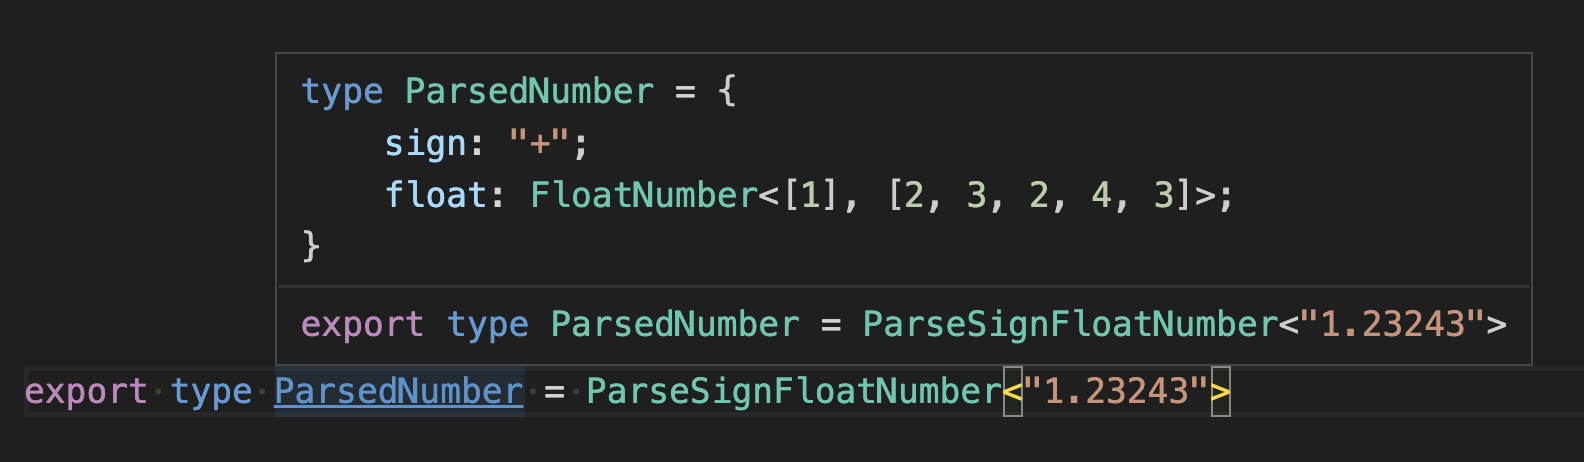
\includegraphics[width=\textwidth]{text/testing/tsserver-hover.png}
  \caption{Inferred type on hover in \acrshort{vscode}}
  \label{fig:tsserver-hover}
\end{figure}

Another key tool used when developing the implementation is the \code{vscode-twoslash-plugin} extension \cite{theroxVscodetwoslashqueries2023}. In order to avoid constantly hovering the cursor on top of symbols to see their inferred types, developers can write the \vcode{// ^?} comment, with the caret pointing to the targeted symbol. The plugin will then display an inlay hint with the inferred type of the selected symbol, as seen in Figure \ref{fig:twoslash-plugin}.

\clearpage

\begin{figure}[ht]
  \centering
  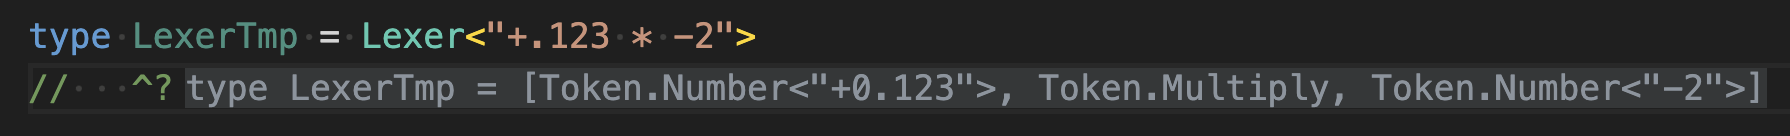
\includegraphics[width=\textwidth]{text/testing/vscode-twoslash-plugin.png}
  \caption{Twoslash syntax of \code{vscode-twoslash-plugin}}
  \label{fig:twoslash-plugin}
\end{figure}

Finally, Pretty TypeScript Errors \cite{balasianoPrettyTypeScriptErrors2023} attempts to parse and reformat the TypeScript error messages to be more human-readable in \acrshort{vscode}. This is especially helpful when dealing with complex object types, where the error messages can become unreadable since the error message and the serialised type is printed out on a single line, as seen in Figure \ref{fig:pretty-ts-errors}.


\begin{figure}[ht]
  \centering
  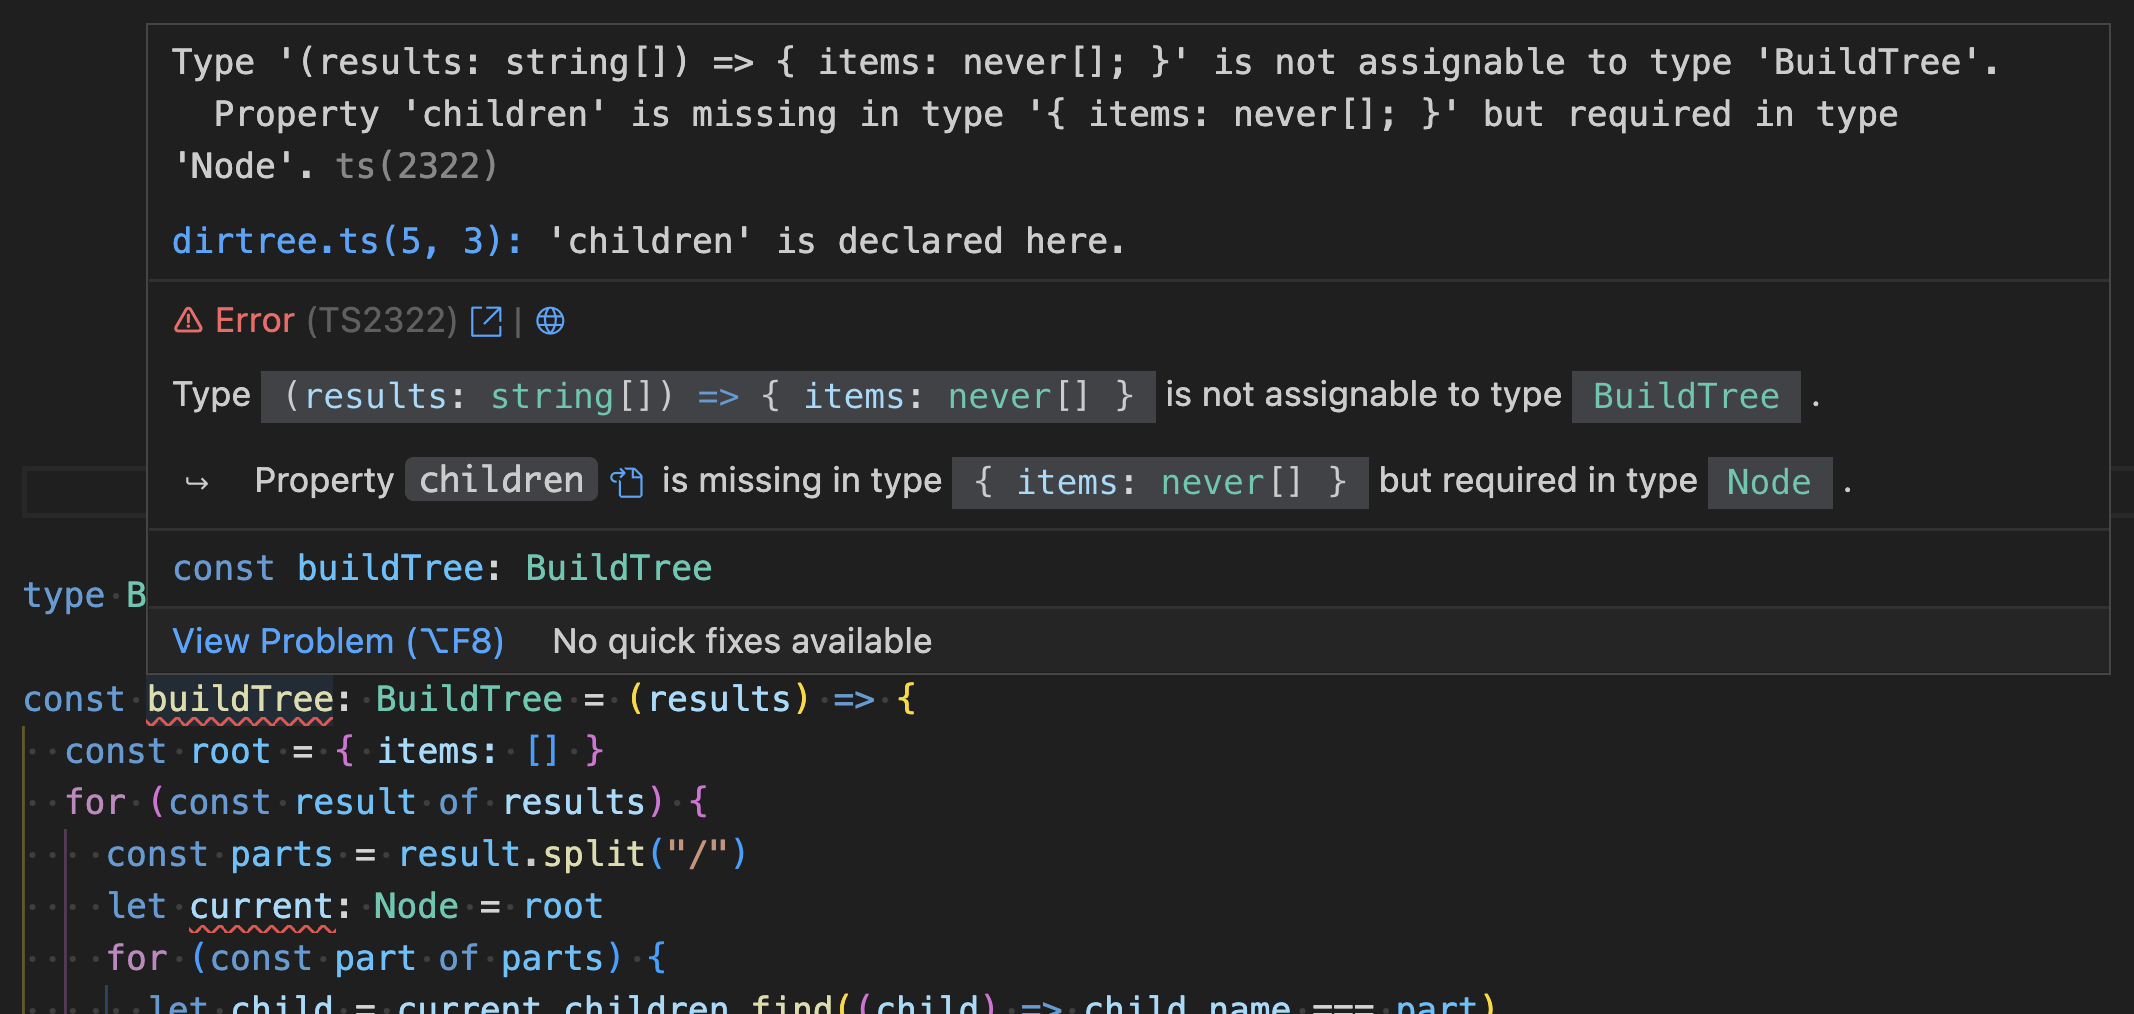
\includegraphics[width=\textwidth]{text/testing/pretty-ts-errors.png}
  \caption{Formatting errors with Pretty TypeScript Errors extension}
  \label{fig:pretty-ts-errors}
\end{figure}

Some generic types include an accompanying unit test to ensure correctness and prevent regression. Testing is backed with \code{eslint} \cite{ESLint2023}, a static code analyser for JavaScript and TypeScript. Configuration-wise, \code{@typescript-eslint/parser} has been set up as the parser used by ESLint for properly analysing TypeScript code, and \code{eslint-plugin-expect-type} has been added for writing type assertions as comments. \code{eslint-plugin-expect-type} enables writing \code{\$ExpectType}, \code{\$ExpectError} and twoslash type assertions (\vcode{// ^?}). An example test assertion can be seen in Listing \ref{lst:expect-type}.

\begin{listing}[ht]
  \begin{minted}{TypeScript}
// $ExpectType "0.3619047620"
type EvaluateCase = Evaluate<
  RecursiveParser.Parse<Lexer<"3.1 + 2.5 * (1 - 5.6) / 4.2">>
>
\end{minted}
  \caption{Type assertion with \code{\$ExpectType}}\label{lst:expect-type}
\end{listing}


\clearpage

\section{CI/CD workflow and release management}

\acrfull{ci} and \acrlong{cd} are the two key parts of the software development process that help developers deliver high-quality software. \acrlong{ci} (\acrshort{ci}) is the practice of automating the integration of code changes into a version control repository \cite{atlassianContinuousIntegrationVs}, encouraging developers to merge their changes to the main branch as often as possible. \acrshort{ci} establishes an automated method for building, packaging and testing the software. The main benefit of this approach is to avoid major integration challenges when releasing a version by continuously integrating more minor changes during the development instead of doing all the integration on the release day.

Whereas \acrlong{cd} (\acrshort{cd}) is an extension of continuous integration, where the code changes are automatically deployed to the production environment after the build and test stage. \acrshort{cd} aims to simplify the deployment as much as possible, making it a routine process that can be performed as many times as needed, even multiple times during a day \cite{WhatCICD}. Note that there is a distinction between Continuous Delivery and Continuous Deployment where the former requires human intervention to deploy changes to production, and the latter is fully automated without any manual steps.

Both Continuous Integration and Continuous Delivery are set up in the implementation part of the thesis. The core of the \acrshort{ci}/\acrshort{cd} setup is the Github Action platform. The GitHub Actions platform allows developers to automate the build, test, and deployment pipeline within an existing GitHub repository \cite{UnderstandingGitHubActions}. The main components of GitHub Actions include workflows, jobs and actions defined using YAML files saved in the \code{.github/workflows}. This project uses two workflows, one for running unit and integration tests and a second one for performing \acrfull{cd} to the \acrshort{npm} registry.

The first workflow, found in \code{.github/workflows/main.yml}, runs both \code{yarn run test} and \code{yarn run build} after every push to the repository event, regardless of branch or reference. The second workflow, found in \code{.github/workflows/publish.yml}, is responsible for handling releases to the \acrshort{npm} registry using Changesets \cite{ChangesetsChangesets2023}. Changesets allow developers to keep track of the release history of a package and automate both versioning and release note generation.

The Changesets tool works by separating versioning into two stages: adding a changeset, describing the changes made in a commit or a branch, and combining created changesets with a version incrementing.

Creation of a changeset is done by running \code{yarn changeset}, which will ask the developer to provide the appropriate version bump type (either MAJOR, MINOR or PATCH, following the Semver versioning) and a message describing the changes. The changeset will be saved as a Markdown file with a unique identifier in the \code{.changesets} folder. The file will be committed to the Git repository. These changesets are preserved in the repository until the release is ready to be published by merging the changesets into the \code{main} branch.

After a push event to the \code{main} branch occurs, the release process, defined as a GitHub Actions job, is launched. The release process itself works by running \code{yarn changeset publish} command and works as such; When new changesets are found in the \code{main} branch, Changesets will automatically create a new pull request, which will perform all of the key steps for releasing a package: incrementing the version, updating the \code{CHANGELOG.md} file and removing the accumulated changelogs. When the pull request is merged, Changesets will automatically publish the new version to the \acrshort{npm} registry and create an appropriate Git tag for the release.

\section{Performance testing}

\begin{itemize}
  \item Difference between operations, execution time + number of created types \code{yarn tsc --noEmit --incremental false --generateTrace trace --extendedDiagnostics --listFiles -p tsconfig.json --explainFiles}
  \item Comparison between other libraries (arielhs/ts-arithmetic)
\end{itemize}



\chapter{Conclusion}

This thesis set out to implement a mathematical expression evaluator entirely written in the type system of TypeScript. Core concepts and techniques of TypeScript type-level programming were introduced and explained. The implementation of the expression evaluator was described in detail, and the implementation was evaluated in terms of correctness and performance using type-level unit tests and benchmarking suites.

The created evaluator is a proof-of-concept, demonstrating the capabilities of the TypeScript type system while addressing some of the limitations of the type system by applying workarounds.

This thesis also provides a comprehensive guide to the TypeScript syntax and type system and can be used as a reference for beginners to the type-level programming in TypeScript. Additional tools and utility types were introduced to aid the development of the mathematical evaluator, namely the benchmarking tool and the LL(1) parser generator.

The rest of this chapter will discuss both the practicality of the created types and the limitations of the type system found during development. Finally, the future work will be outlined.

\section{Practical usage}

The TypeScript type system is powerful for static type-checking and inference. However, it is not without its limitations. These advanced types are considered to be extreme and are generally not recommended to be used in production code, as they can severely impact the compilation time and the in-editor developer experience.

Nevertheless, there are some possible practical use cases for these advanced types. Literal types are often used to describe a design system and accompanying design tokens. Namely, numeric literal types are used to describe the spacing and sizing of components. When the spacing is defined in other units, such as \code{rem} or \code{em}, developers often need to manually convert the values into pixels. A utility type can be introduced to convert values in \code{rem} or \code{em} units into pixels and reverse. This can be further expanded to allow more type transformations, such as converting a Tailwind CSS class name into a CSS string without any TypeScript editor plugins.

The parser and the accompanying parser generator can accept any LL(1) grammar and can be used to parse more complex formats, such as JSON. Finally, the benchmarking tool can be used to benchmark any type-level code in isolation, keeping all the test cases in a single file.

\section{Limitations of the TypeScript type system}

When developing the implementation of the evaluator, some limitations of the TypeScript type system were discovered.

In general, error messages in TypeScript are suboptimal. They tend to be displayed in one line without any formatting, and if they include complicated types, the types are truncated, which leads to a suboptimal debugging experience. Even with \code{noErrorTruncation} flag turned on in \code{tsconfig.json}, the type message is still truncated due to a hard limit. The limit can be artificially raised by patching the TypeScript source code, namely by increasing the \code{defaultMaximumTrucationLength} limit, but this is not a viable solution for production code. The only other option is to manually recreate intermediate types when debugging complicated types.

The type checker itself contains many hardcoded constraints to prevent performance degradation, ranging from the maximum tuple size to the limit on both instantiation count and depth. Some checks can be bypassed using various workarounds, often at a performance cost, discussed in previous chapters. However, these workarounds are poorly documented in the official TypeScript documentation and can break with new TypeScript releases without further notice.

Even though the TypeScript type system is powerful for complex types, some highly requested features are still missing as of the writing of this thesis, such as the lack of partial type argument inference \cite{ImplementPartialType} or lack of built-in utility types for type-level assertions. Some of these features can be partially emulated, such as the lack of higher kinded types, but the behaviour can also change with new TypeScript releases.

Finally, as the type checker itself is written in TypeScript to dogfood the language, it can be inherently slow when working with larger TypeScript codebases. Some of these performance issues are being solved by rewriting the type checker in a different programming language, such as Rust \cite{Stc2023}, but the project is still under active development.

\section{Future work}

Most of the future work is geared towards the underlying tooling and utilities rather than the mathematical expression evaluator itself, which can be further extended by adding additional mathematical operations based on the existing utility types implemented in this thesis.

For instance, the LL(1) parser generator is not flexible enough, as it can only generate code for LL(1) grammars, which, while being sufficient for mathematical expressions and other simple formats such as JSON, is not enough for more complex grammars. Future work could include creating a more generic Look-Ahead LR parser generator, which would be able to parse more complex grammars and programming languages.

The benchmarking utility itself can be extended and packaged both as an \acrshort{npm} package and as a GitHub Action. This is especially useful for library maintainers, which can use the additional CI step to monitor potential performance regressions when reviewing pull requests from contributors.


\appendix\appendixinit % do not remove these two commands

\backmatter % do not remove this command

\printbibliography % print out the BibLaTeX-generated bibliography list

\chapter{Contents of the attached media}


\dirtree{%
.1 .changeset.
.2 config.json\DTcomment{Configuration file for Changesets}.
.1 .github.
.2 workflows.
.3 main.yml\DTcomment{Continuous integration and testing}.
.3 publish.yml\DTcomment{Automatic publishing to \acrshort{npm} registry}.
.1 .vscode\DTcomment{Common configuration for VSCode}.
.1 assets\DTcomment{Assets for \acrshort{npm} and GitHub README}.
.1 benchmark\DTcomment{JSON benchmarking results}.
.1 scripts.
.2 bench.ts\DTcomment{Benchmarking script}.
.2 dirtree.ts\DTcomment{Generator of LaTeX dirtree}.
.2 generate.ts\DTcomment{Lookup table generation}.
.2 parser.ts\DTcomment{LL(1) parser generator}.
.1 src\DTcomment{Source code of the implementation}.
.2 expression\DTcomment{Expression evaluator}.
.2 math\DTcomment{Mathematical operations}.
.2 utils\DTcomment{Utility functions}.
.1 thesis\DTcomment{Source code for the thesis}.
}
 % include `medium.tex' from `text/' subdirectory

\end{document}